% !TeX spellcheck = en_GB
\section{Control Plots}\label{section:star_nonSD}
\begin{comment}
The background contributions coming from \ac{ND}, \ac{DD} and \ac{CD} events are estimated from \ac{MC} simulations. Protons from elastic interactions and beam halo are not included in the~simulation. \ac{SD} background signatures which are modeled in th~\ac{MC} simulations are only coming from :
\begin{itemize}
\item forward protons produced in the \ac{SD}, \ac{CD} or \ac{DD} diffractive systems or through non-diffractive  \ac{QCD},
\item reconstructed tracks coming from showering.
\end{itemize}

Figure~\ref{fig:nonSDxit} shows the uncorrected $\xi$ and $t$ distributions in data compared to various \ac{MC} models: PYTHIA 8 A2 (MBR), PYTHIA 8 A2 (MBR-tuned) and EPOS. The \ac{MC} distributions are split into \ac{SD}, \ac{ND}, \ac{DD} and \ac{CD} components. For EPOS low mass excitation of the proton remnant (SD') is separated from the ND events. Additionally, the accidental background is also shown. Without arbitrary suppression of diffractive cross sections at large $\xi$ PYTHIA8 A2 (MBR-tuned) predictions agree much better with the data and result also in a suppression of non-SD events. EPOS describes data better than PYTHIA8 but shows a dominant contribution of SD' events. All MCs predict significant non-SD background at large $\xi$, thereby  the analysis was limited to $\xi < 0.2$. 

On the other hand, \cref{fig:nonSDnsel,fig:nonSDpt,fig:nonSDera} show the uncorrected distributions of variables used in the later analysis: $n_{\mathrm{sel}}$, $p_{\mathrm T}$ an $\bar{\eta}$. The background contributions from non-SD interactions differ a bit between each other, i.e. EPOS predicts significantly larger CD contribution, whereas DD and ND are suppressed in PYTHIA 8 A2 (MBR-tuned).  As a result PYTHIA~8~A2~(MBR) is used as the default model  of non-SD with systematic uncertainty $\pm50\%$, which covers all differences between the~models. %Moreover, SD' in EPOS was not subtracted but used separately for comparisons.

\begin{figure}[H]
\centering
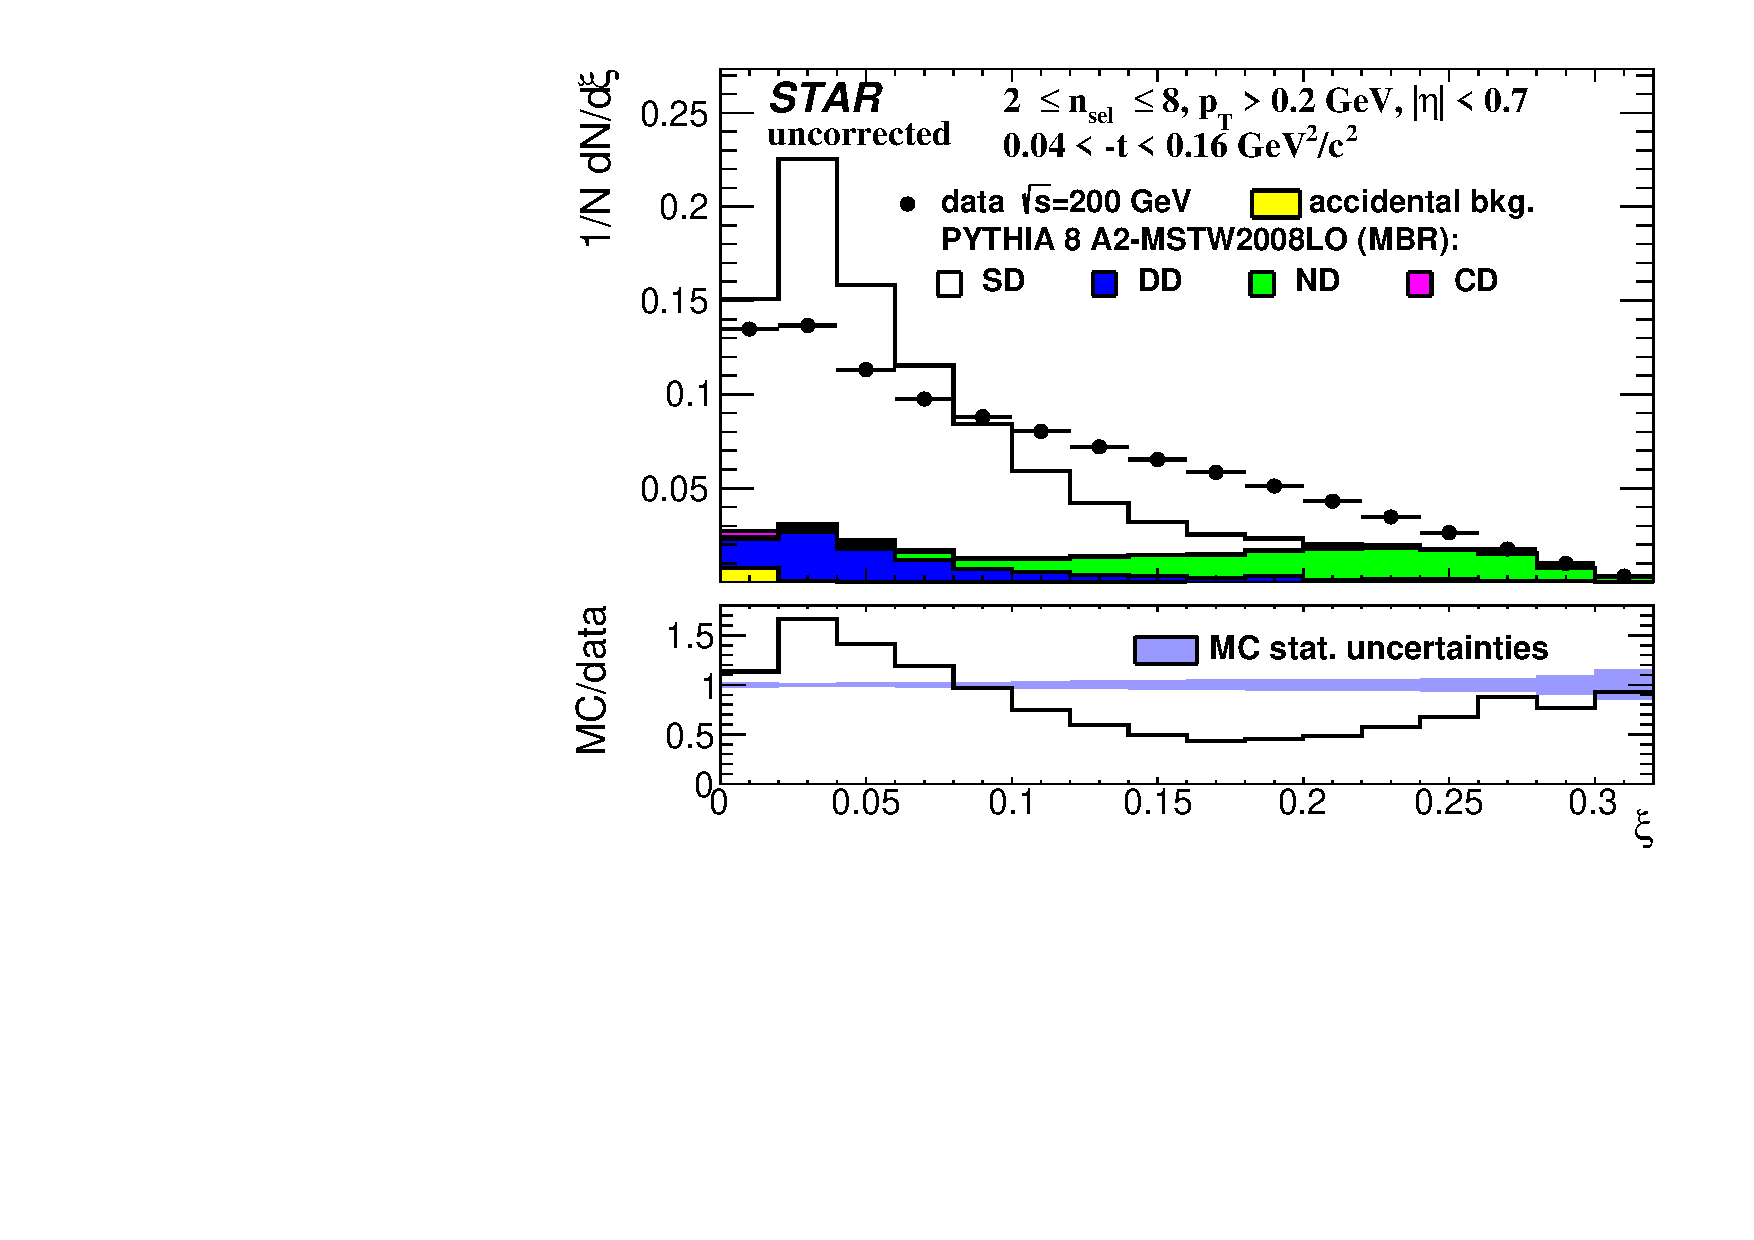
\includegraphics[width=.49\textwidth,page=1]{chapters/chrgSTAR/img/nonSD/SDT_pythia_xi0_RP_starsim_xi.pdf}
\hfill
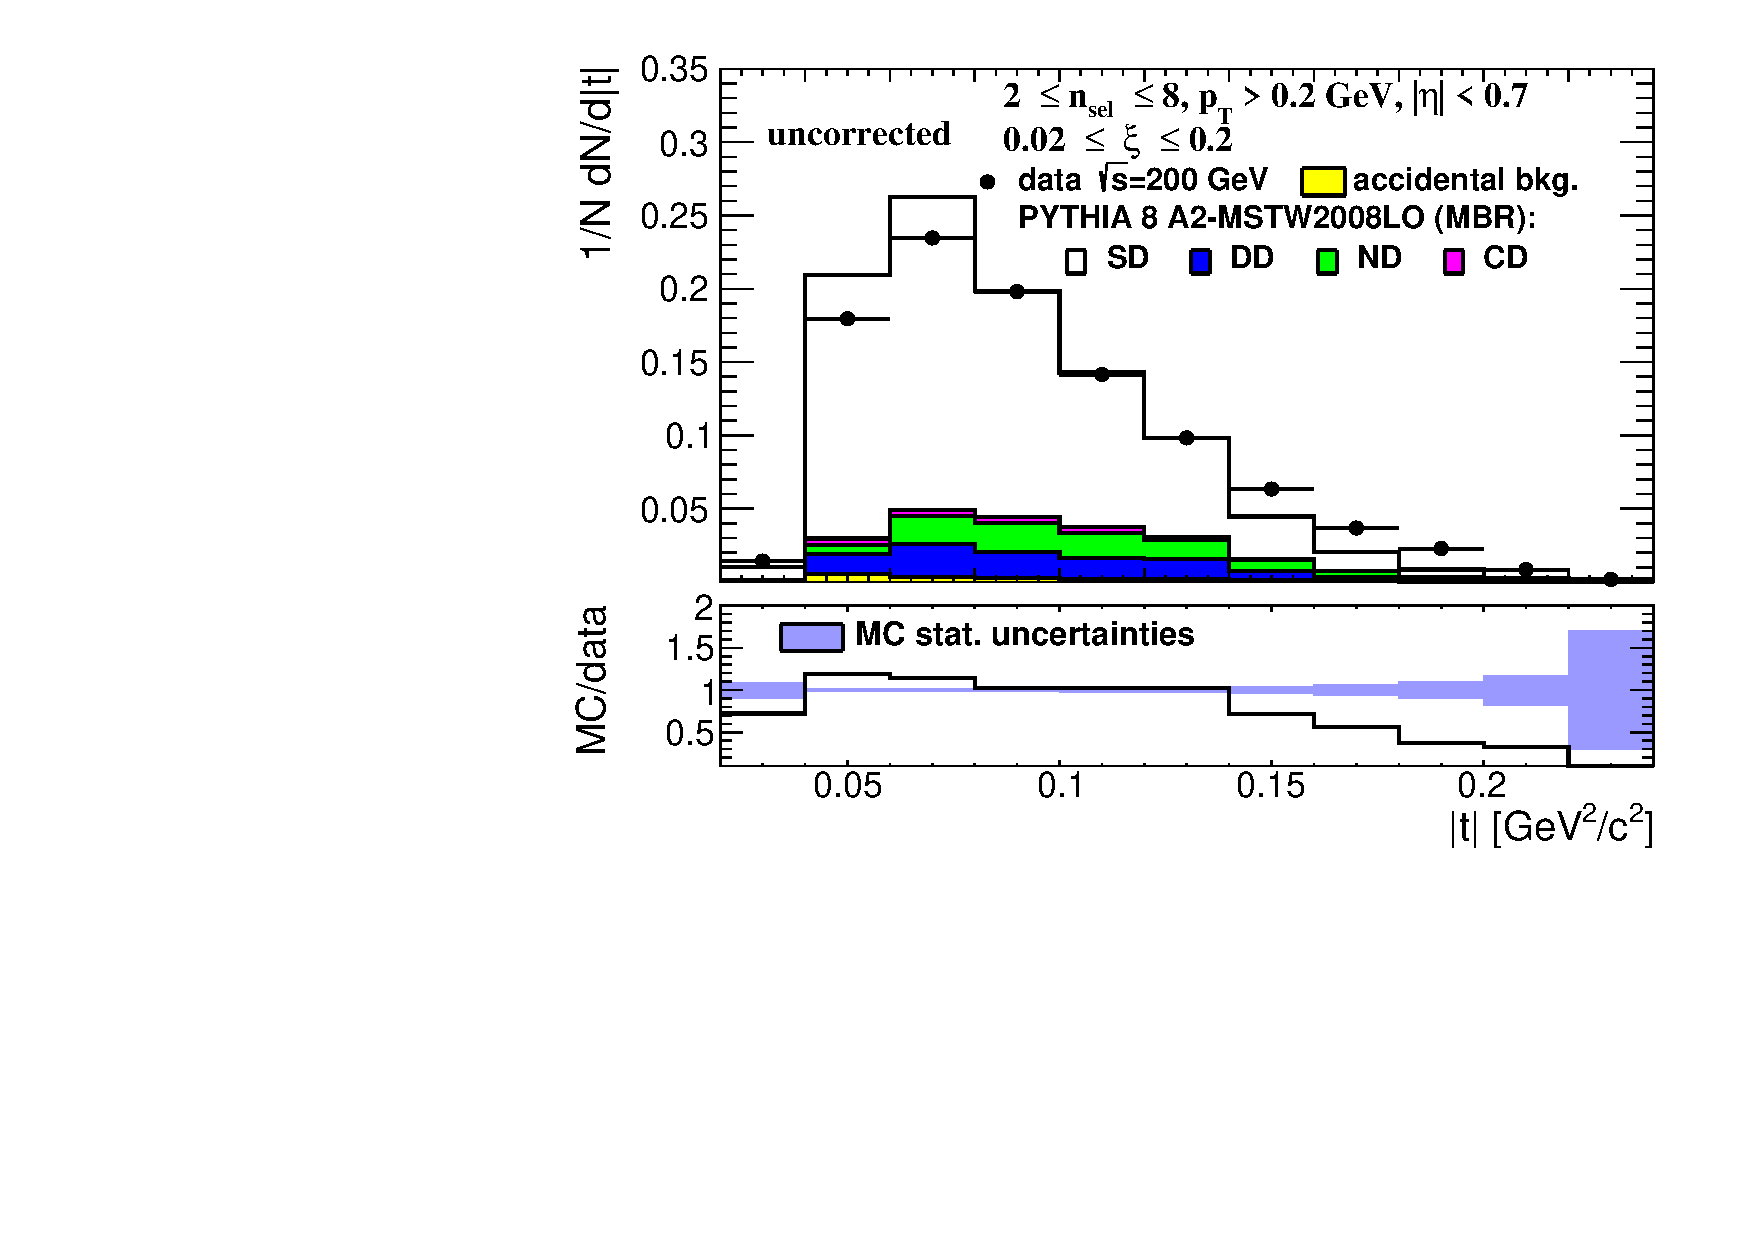
\includegraphics[width=.49\textwidth,page=1]{chapters/chrgSTAR/img/nonSD/SDT_pythia_xi0_RP_starsim_t.pdf}
\newline
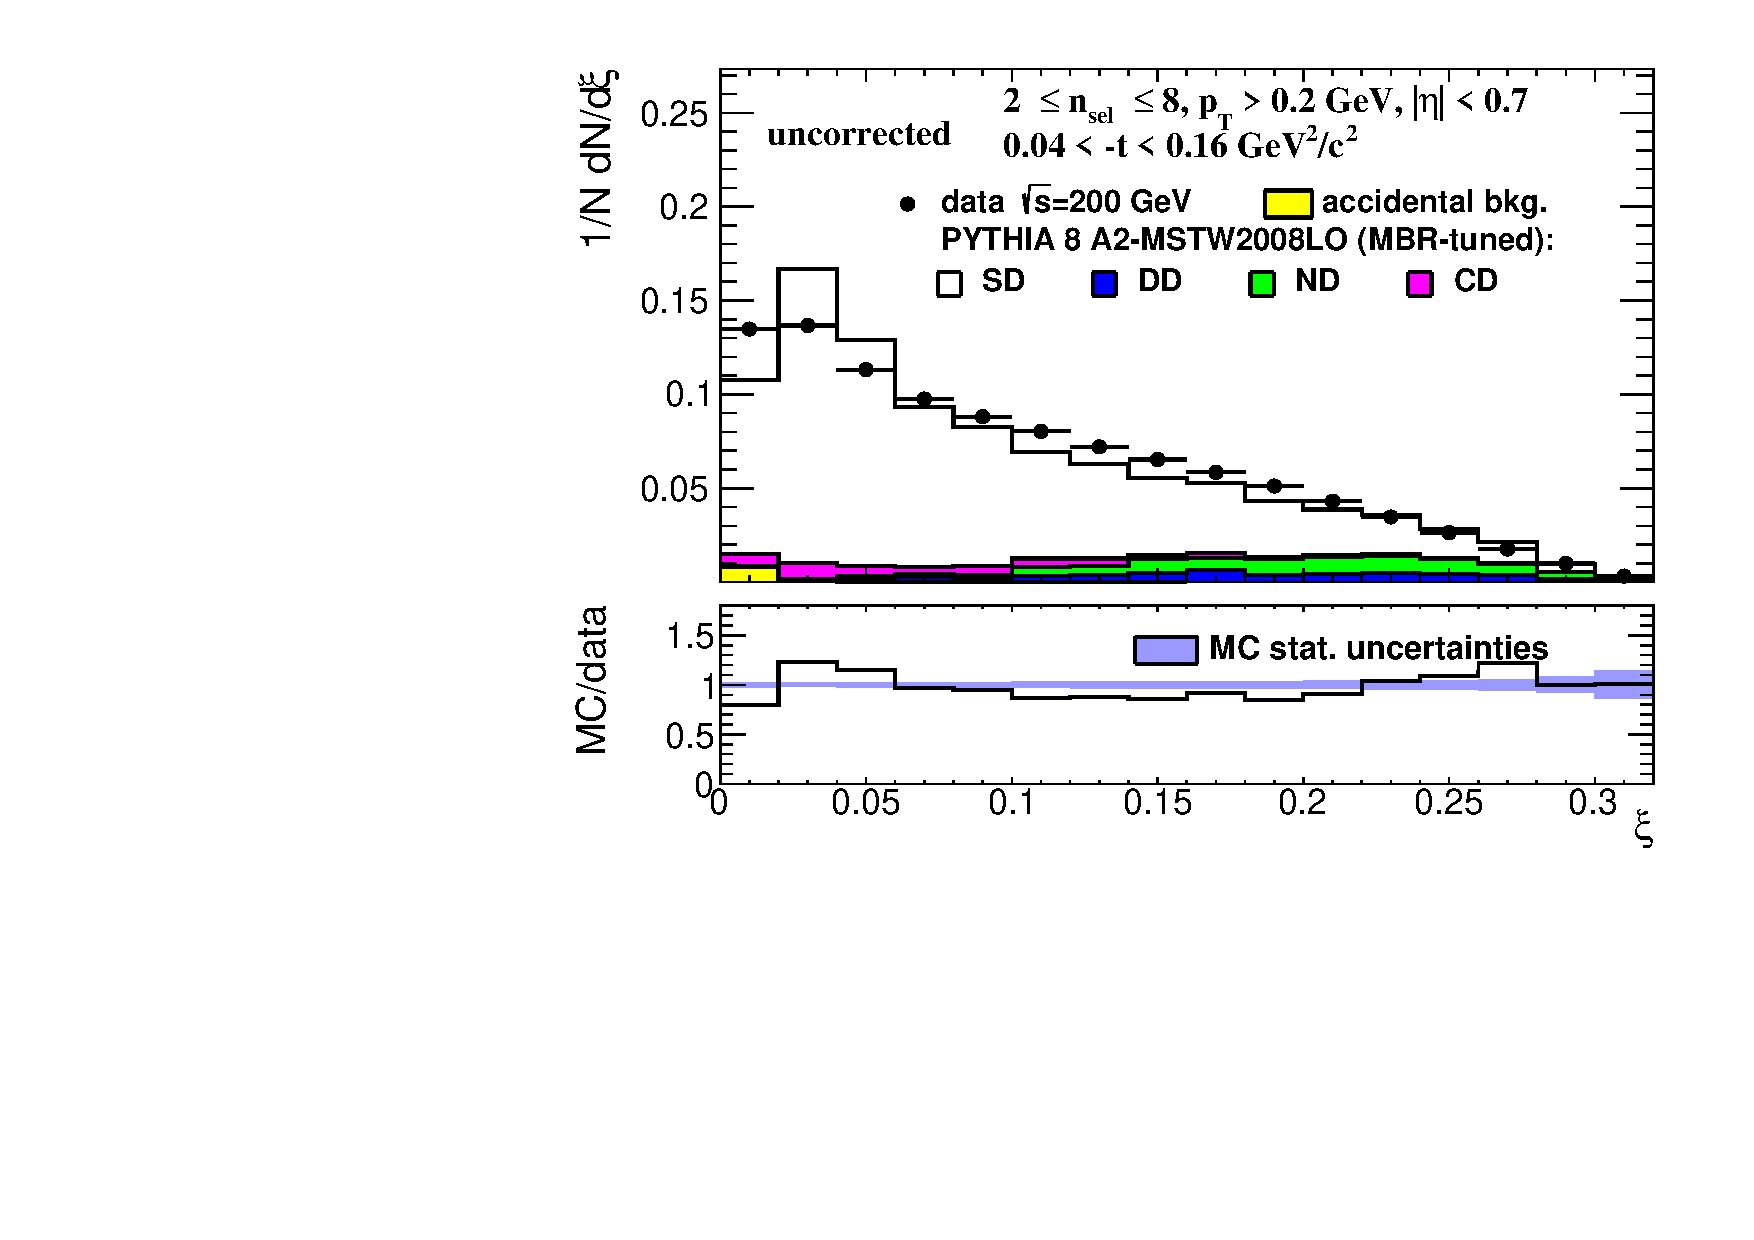
\includegraphics[width=.49\textwidth,page=1]{chapters/chrgSTAR/img/nonSD/SDT_pythia_xi0_option2_RP_starsim_xi.pdf}
\hfill
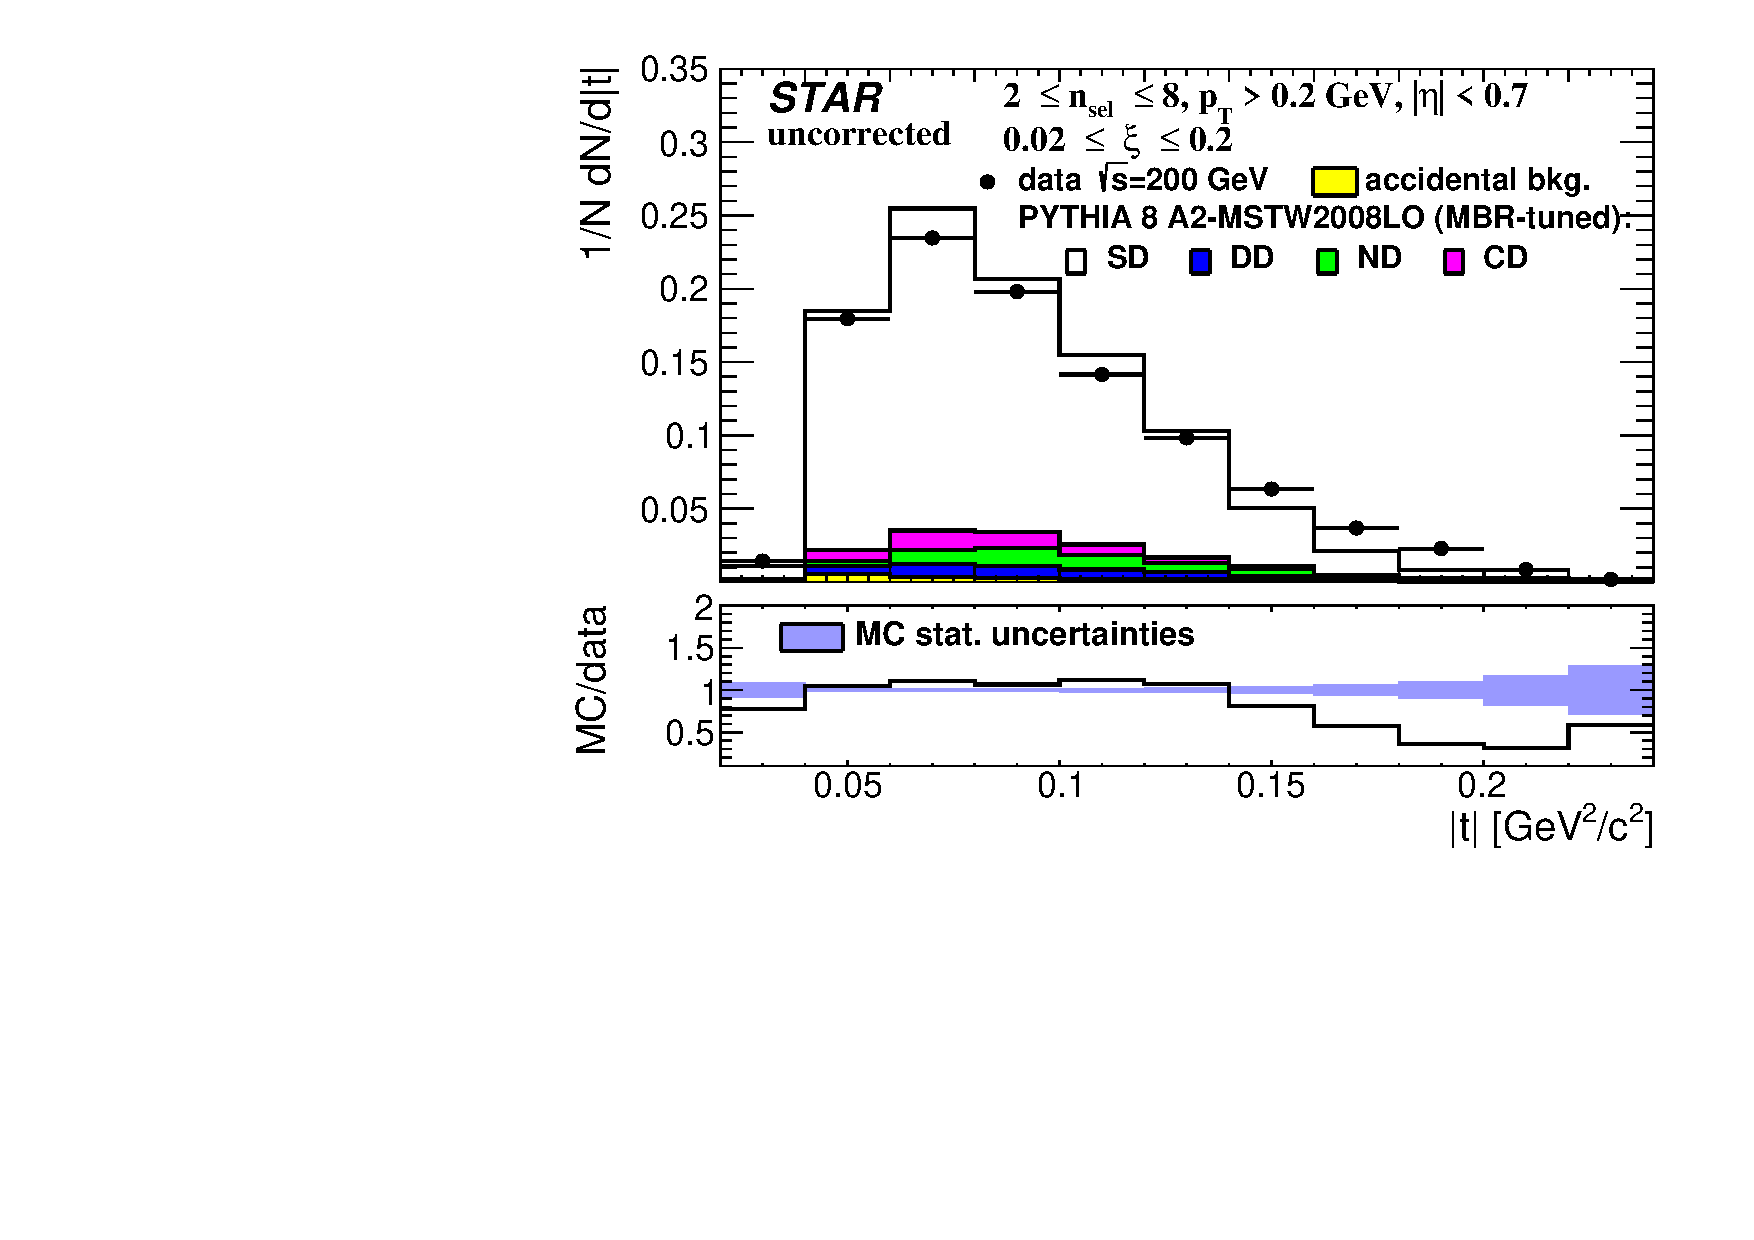
\includegraphics[width=.49\textwidth,page=1]{chapters/chrgSTAR/img/nonSD/SDT_pythia_xi0_option2_RP_starsim_t.pdf}
\newline
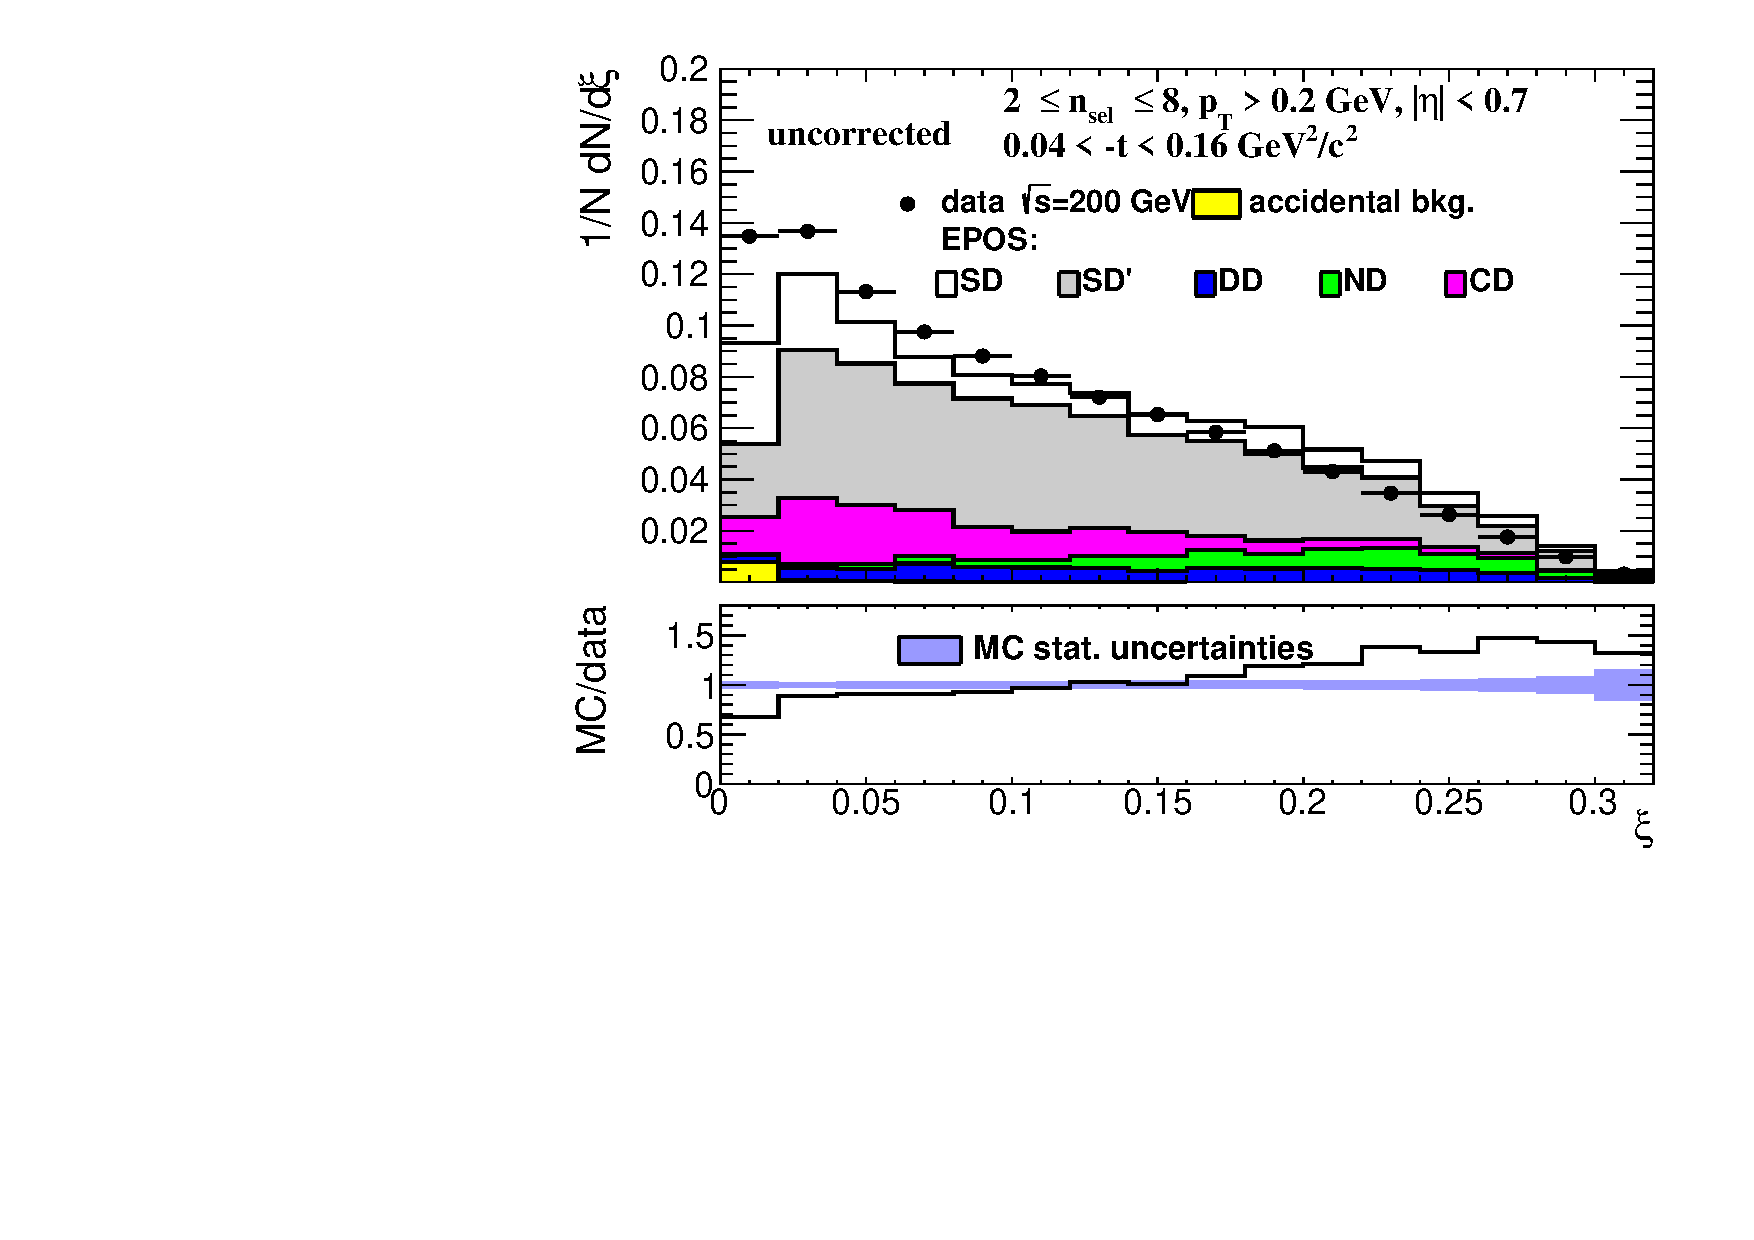
\includegraphics[width=.49\textwidth,page=1]{chapters/chrgSTAR/img/nonSD/SDT_epos_xi0_RP_starsim_xi.pdf}
\hfill
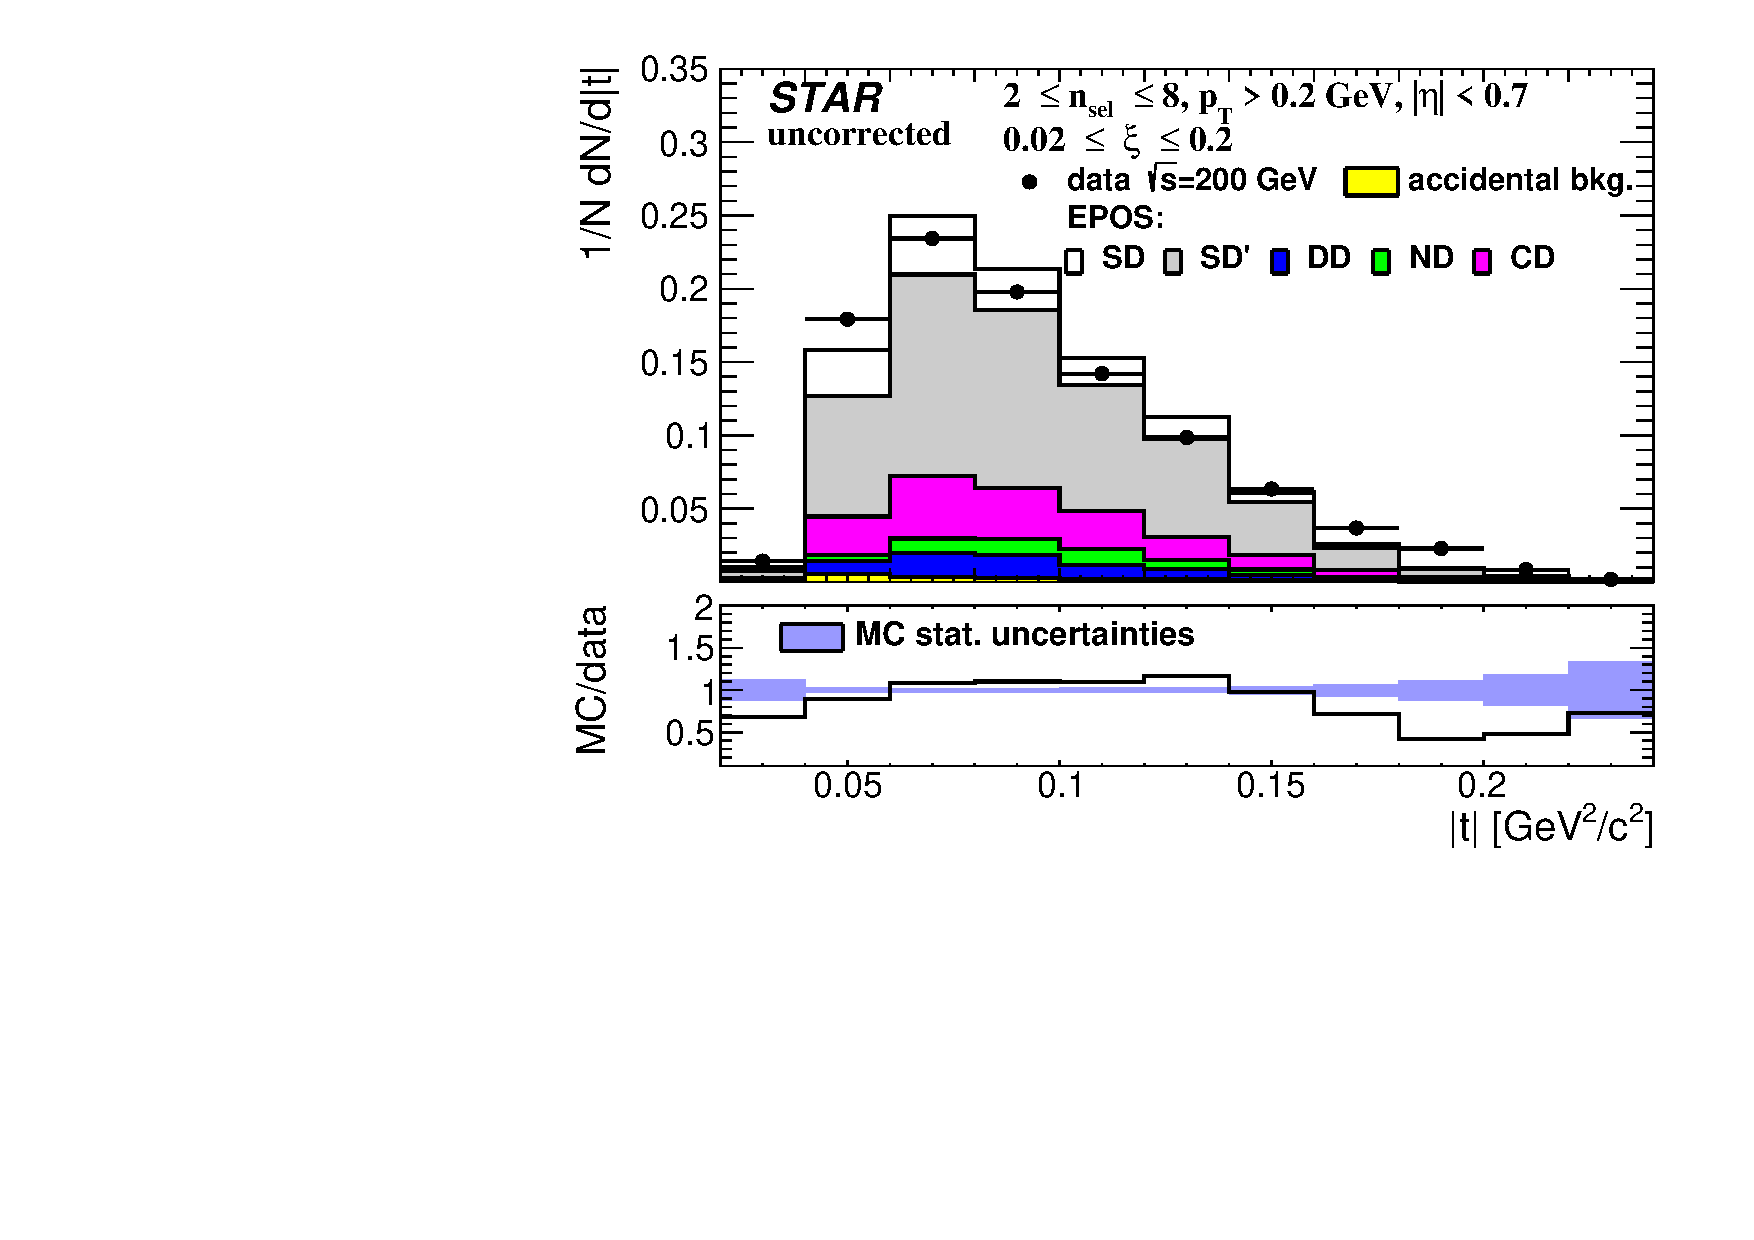
\includegraphics[width=.49\textwidth,page=1]{chapters/chrgSTAR/img/nonSD/SDT_epos_xi0_RP_starsim_t.pdf}
%
\caption{Uncorrected distributions of data compared to various MC models: (top) PYTHIA8 A2 (MBR), (middle) PYTHIA8 A2 (MBR-tuned) and (bottom) EPOS, as a function of (left column) $\xi$  and (right column) $|t|$.}
\label{fig:nonSDxit}
\end{figure}
\newpage

\begin{figure}[H]
\centering
\begin{subfigure}{.45\textwidth}
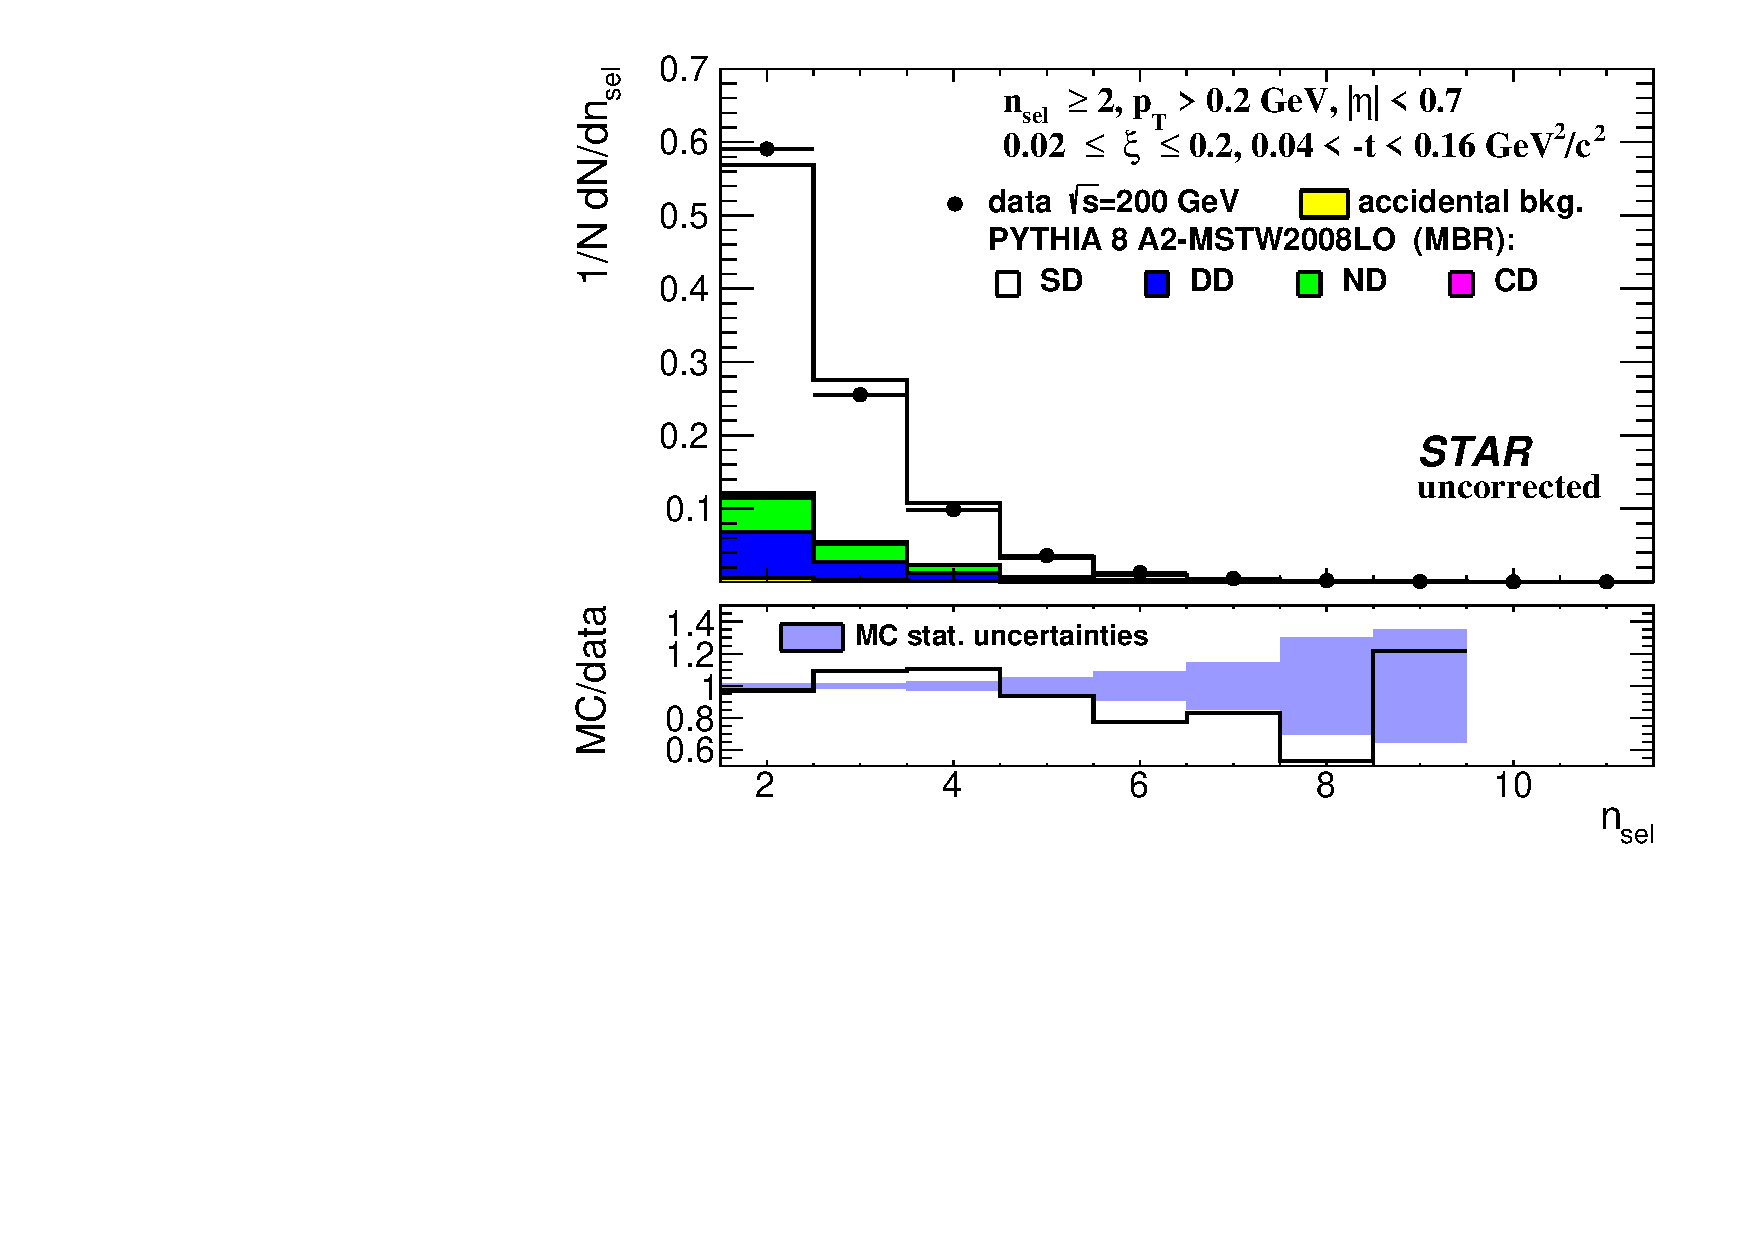
\includegraphics[width=\linewidth, page=1]{chapters/chrgSTAR/img/nonSD/chrg/SDT_pythia_xi0_RP_starsim_nsel.pdf}
\end{subfigure}
\begin{subfigure}{.45\textwidth}
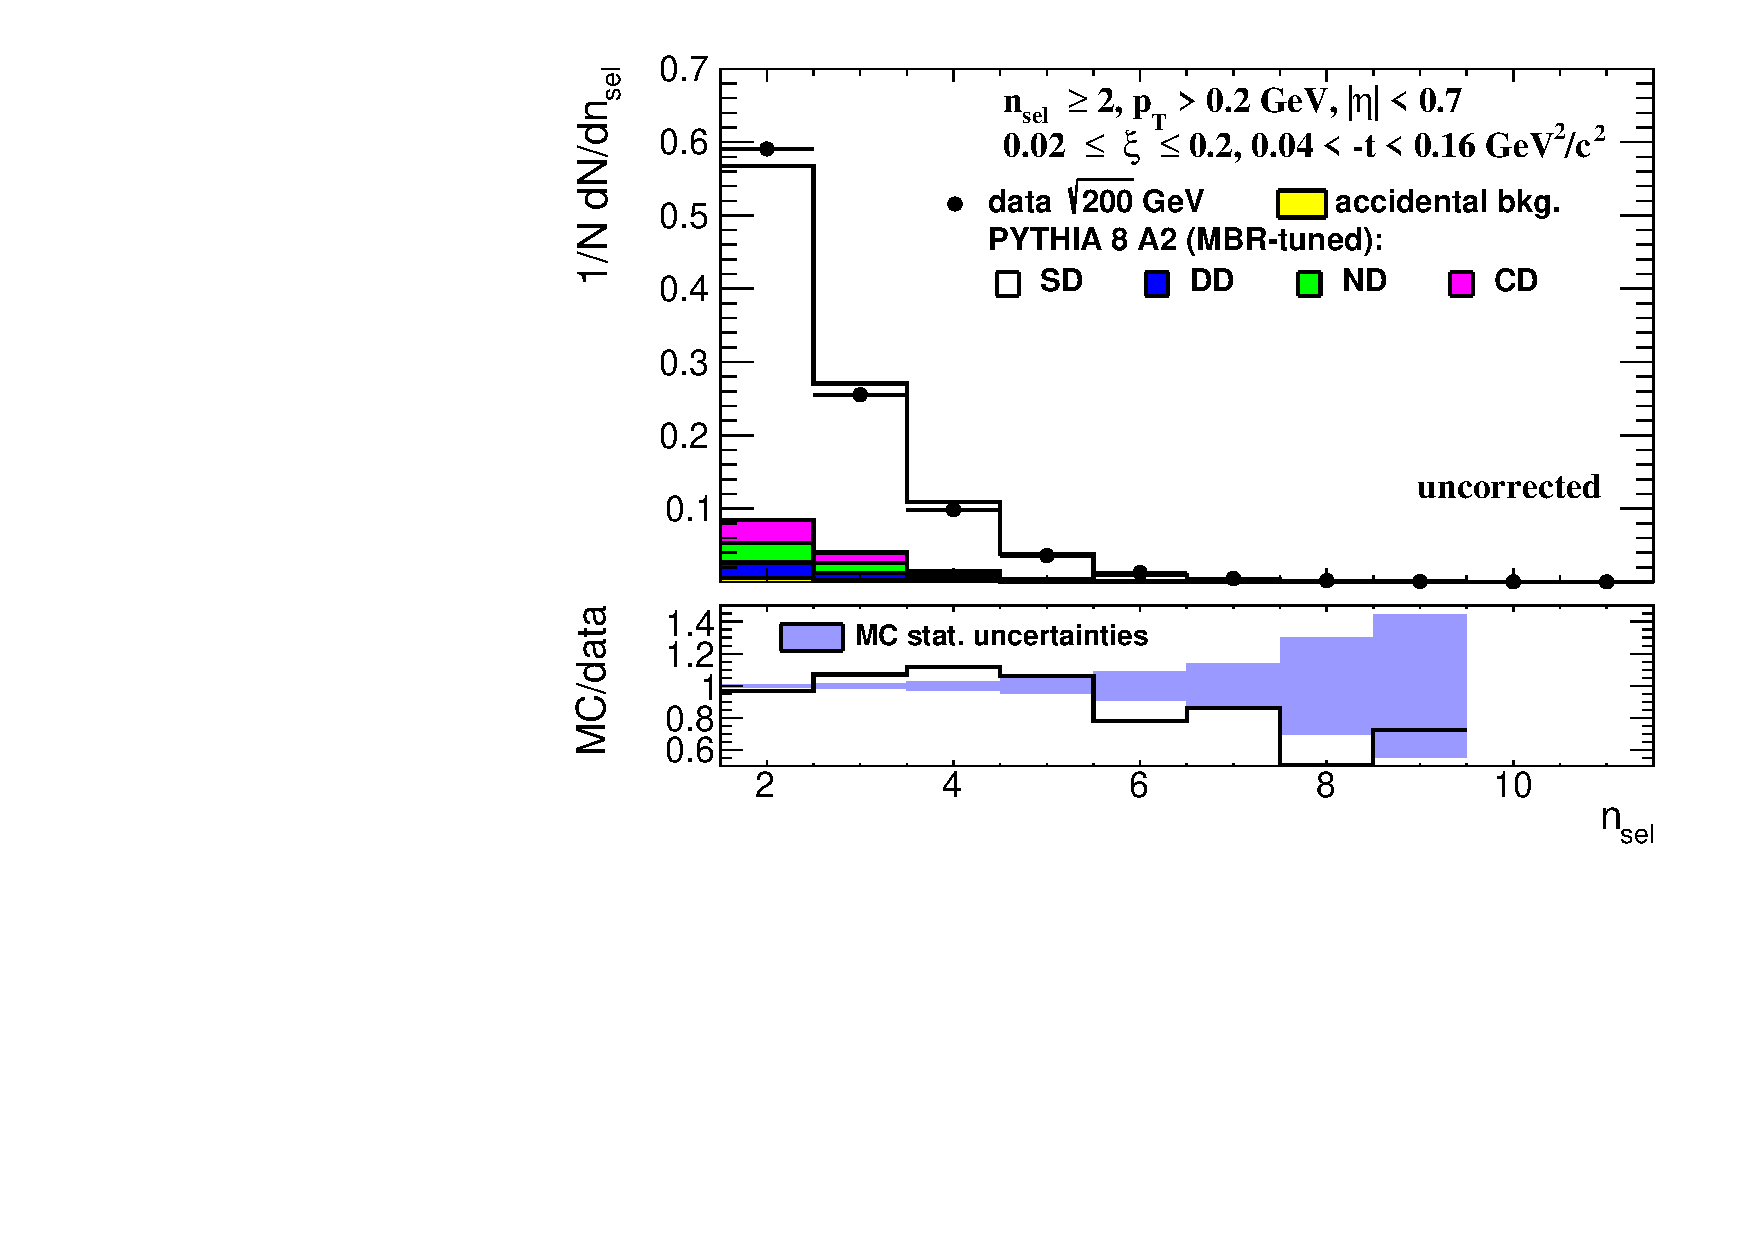
\includegraphics[width=\linewidth, page=1]{chapters/chrgSTAR/img/nonSD/chrg/SDT_pythia_xi0_option2_RP_starsim_nsel.pdf}
\end{subfigure}
\begin{subfigure}{.45\textwidth}
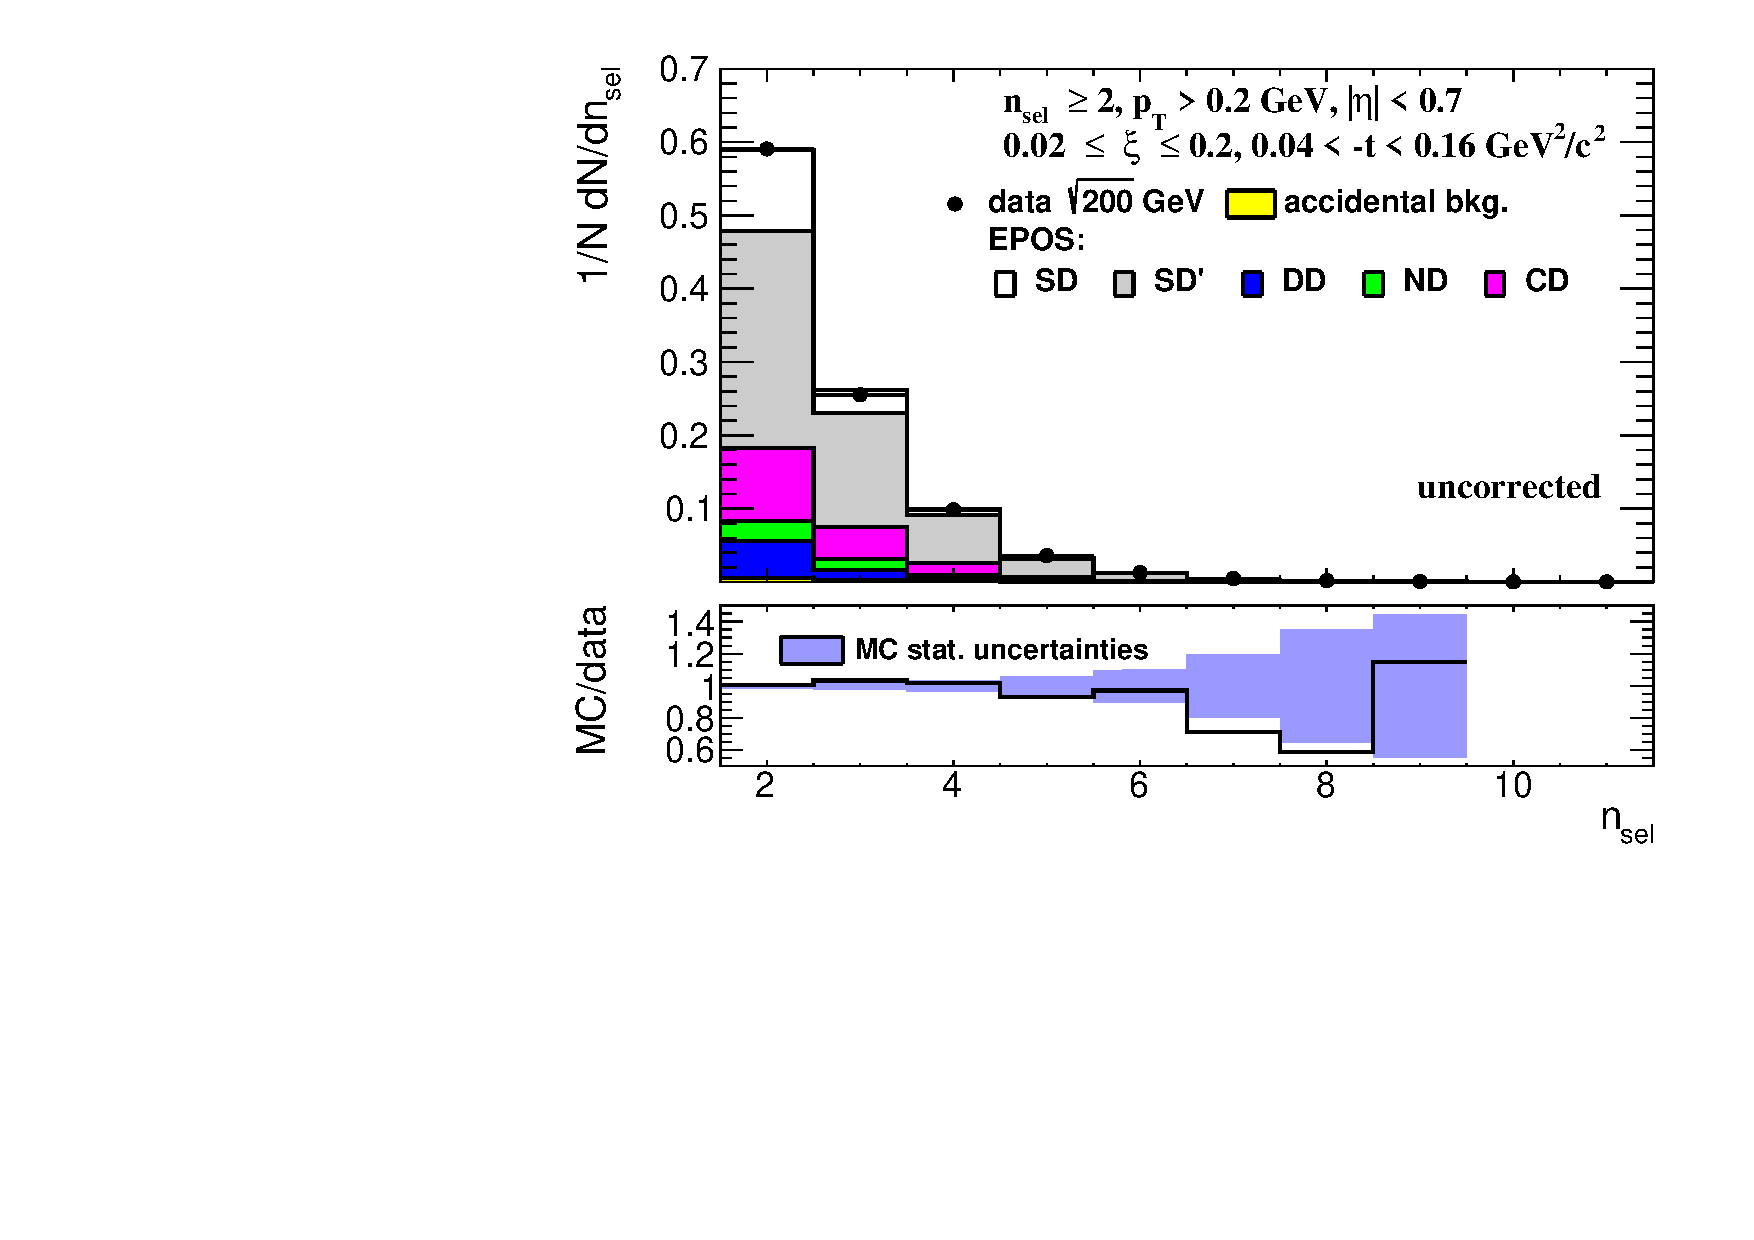
\includegraphics[width=\linewidth, page=1]{chapters/chrgSTAR/img/nonSD/chrg/SDT_epos_xi0_RP_starsim_nsel.pdf}
\end{subfigure}
\begin{minipage}{.45\textwidth}
\caption{Uncorrected distributions of data compared to various MC models: (top left) PYTHIA8 A2 (MBR), (top right) PYTHIA8 A2 (MBR-tuned) and (bottom) EPOS, as a function of $n_{\mathrm{sel}}$.}
\label{fig:nonSDnsel}
\end{minipage}

\end{figure}
\begin{figure}[H]
%	\vspace{-0.5cm}
\centering
\begin{subfigure}{.45\textwidth}
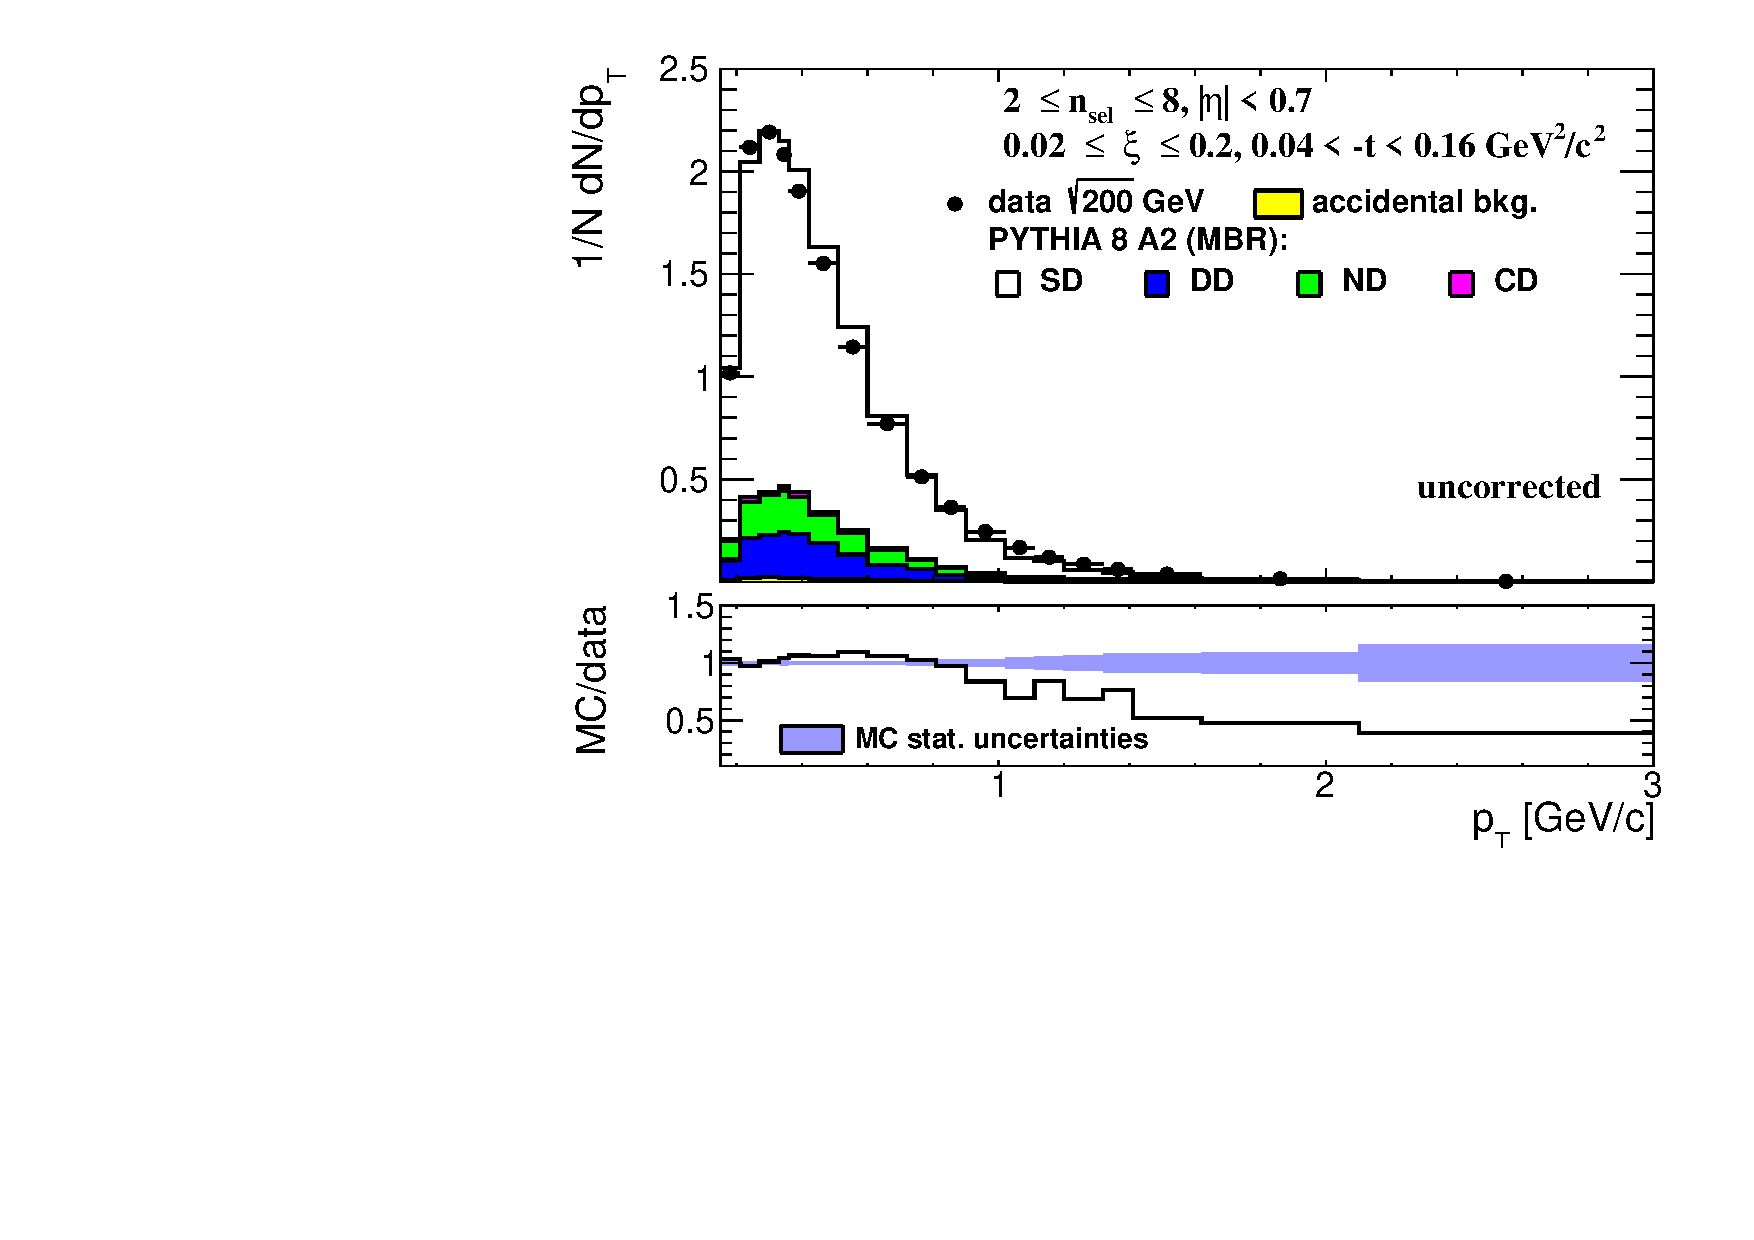
\includegraphics[width=\linewidth, page=1]{chapters/chrgSTAR/img/nonSD/chrg/SDT_pythia_xi0_RP_starsim_pt.pdf}
\end{subfigure}
\begin{subfigure}{.45\textwidth}
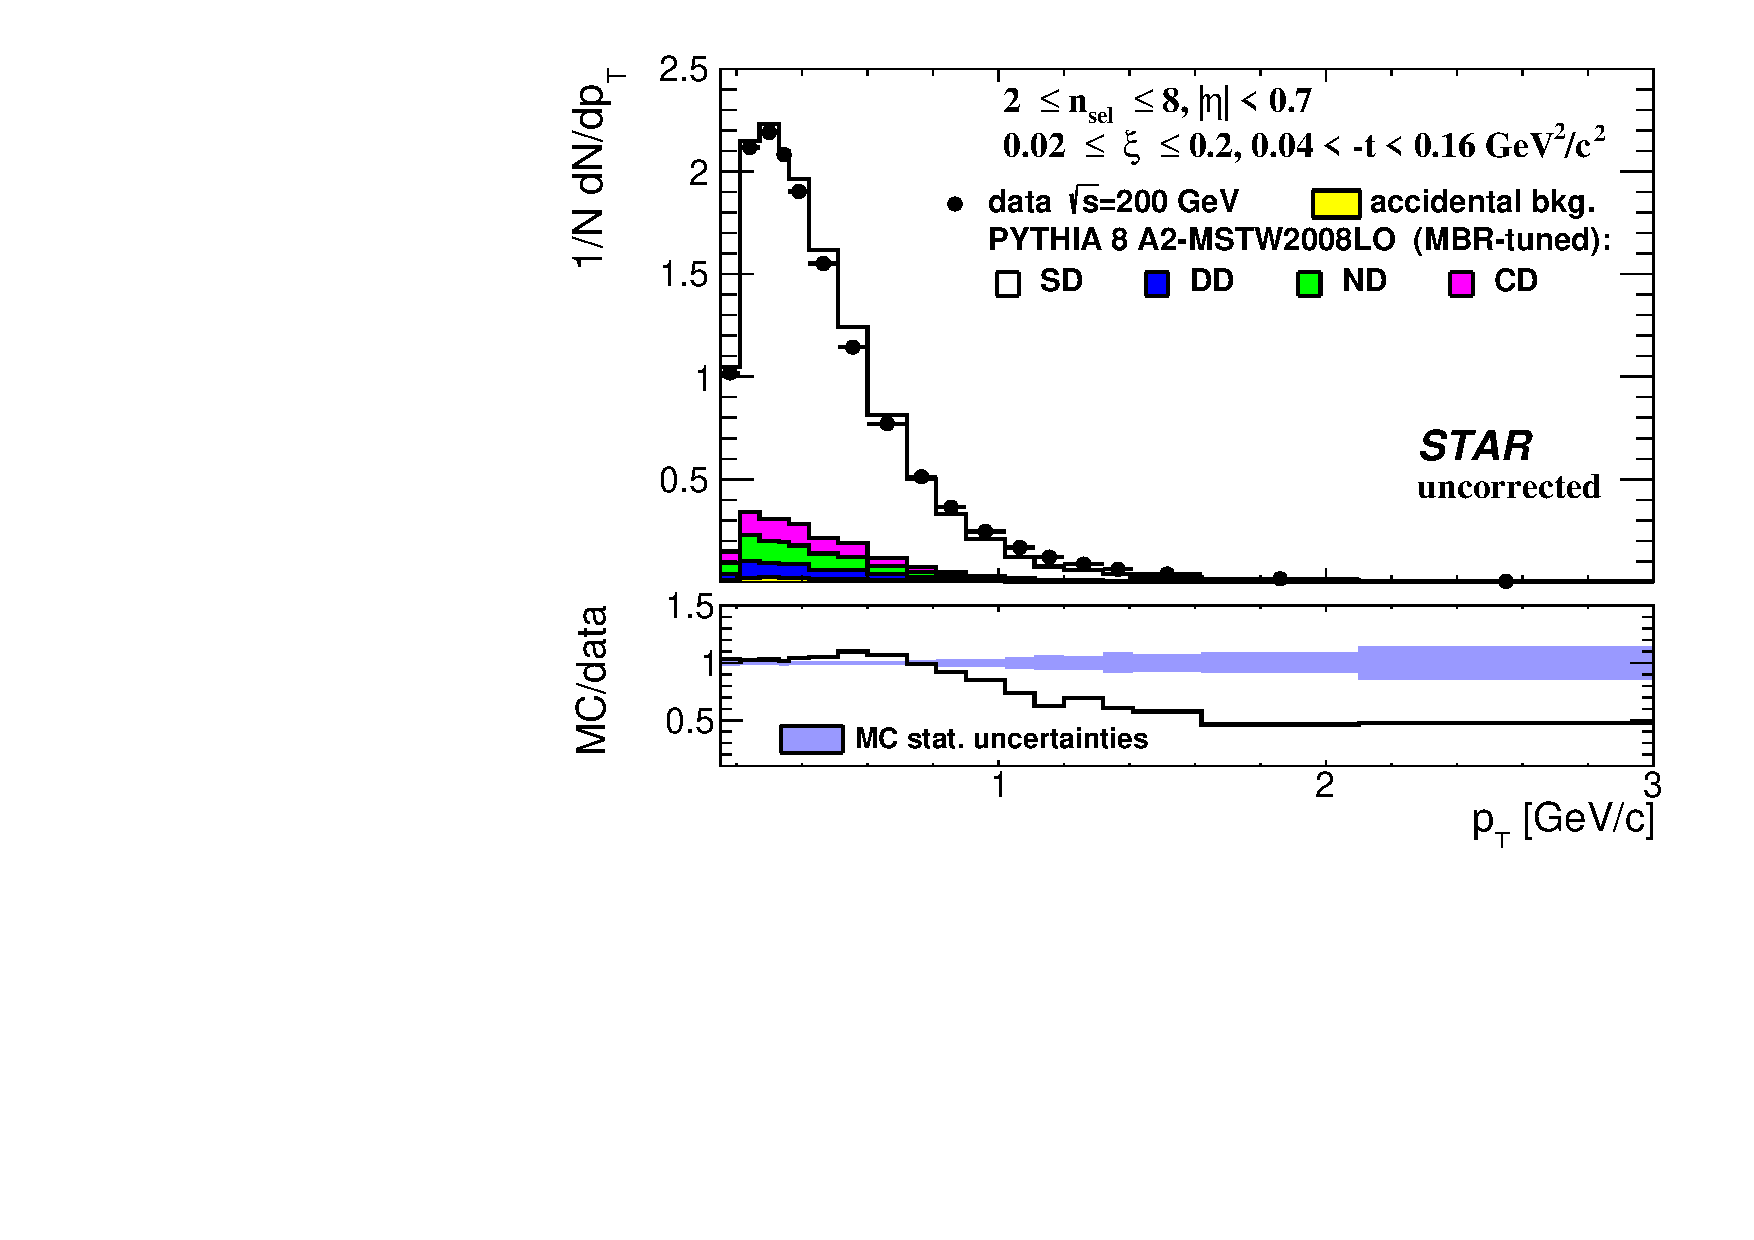
\includegraphics[width=\linewidth, page=1]{chapters/chrgSTAR/img/nonSD/chrg/SDT_pythia_xi0_option2_RP_starsim_pt.pdf}
\end{subfigure}
\begin{subfigure}{.45\textwidth}
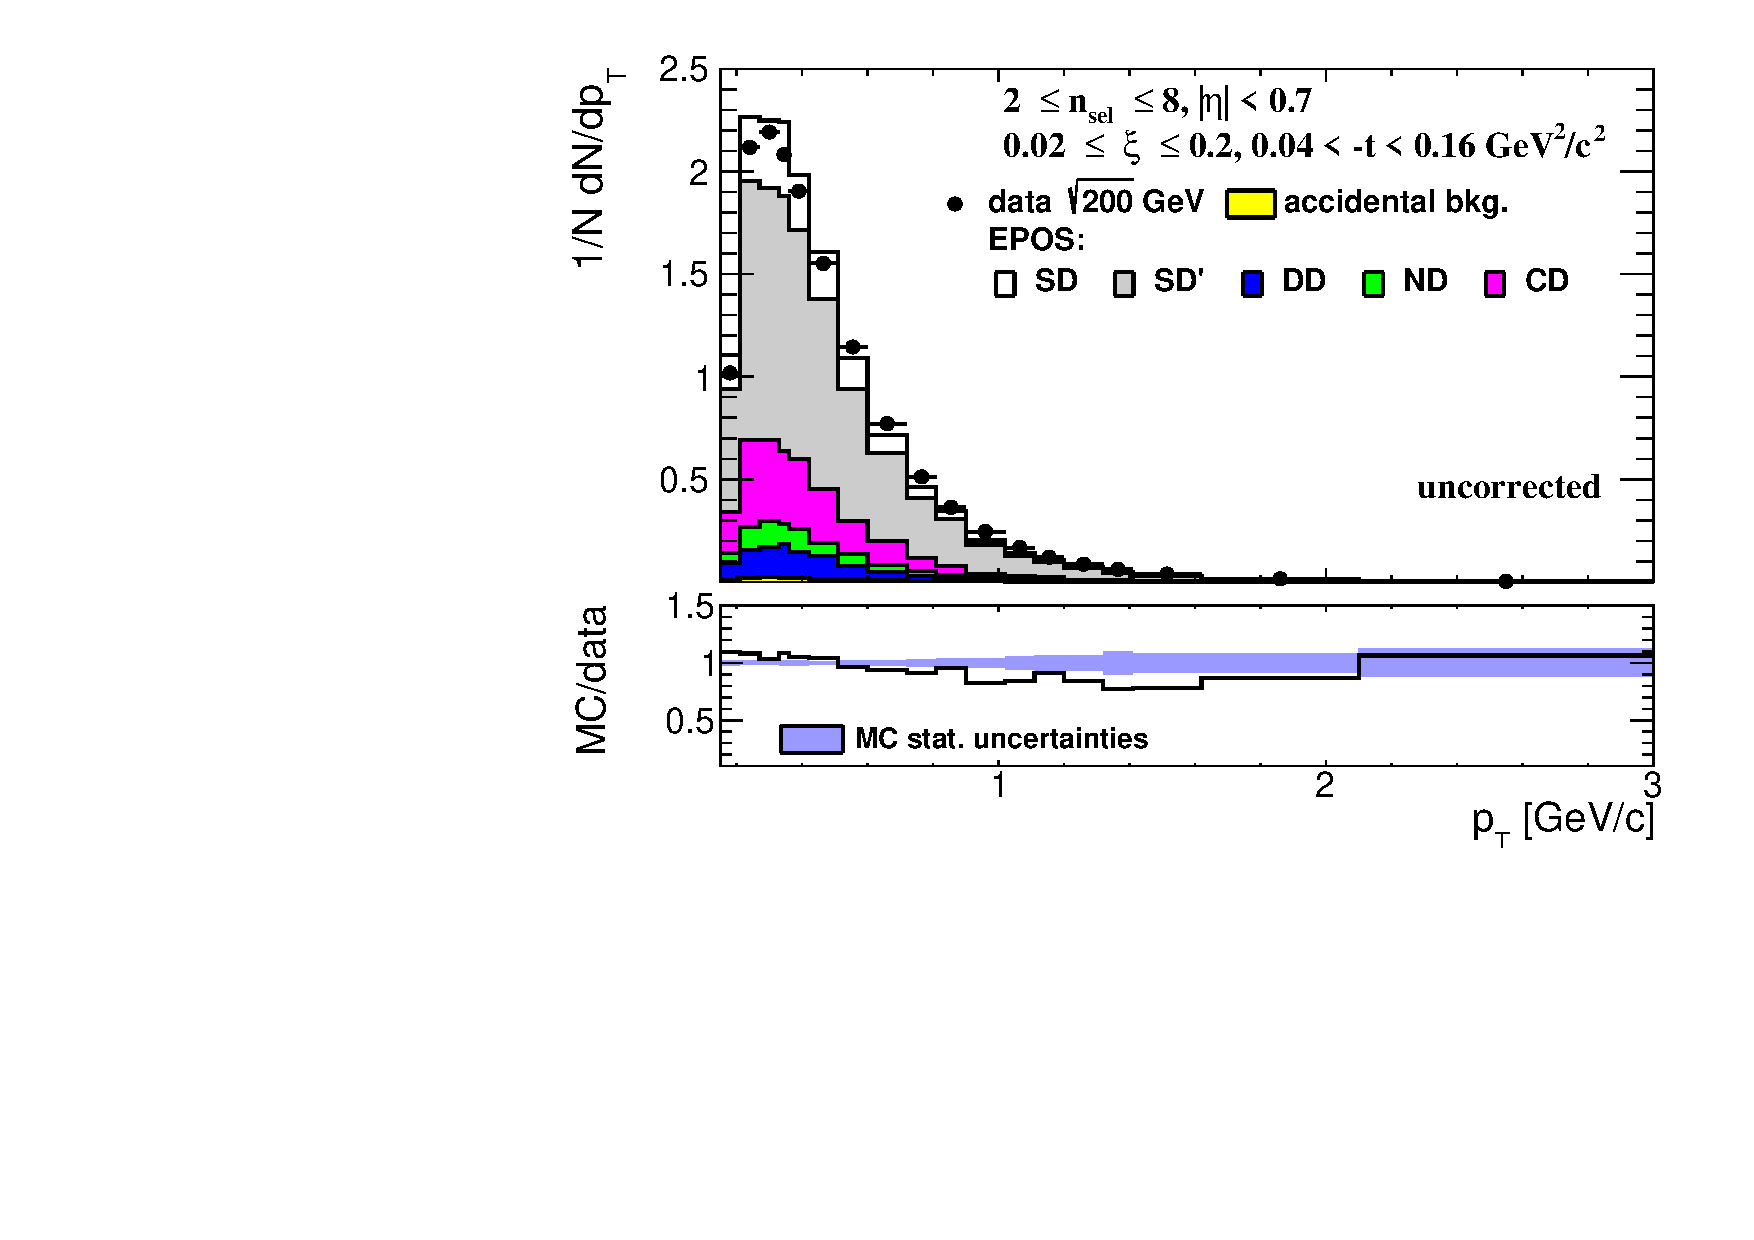
\includegraphics[width=\linewidth, page=1]{chapters/chrgSTAR/img/nonSD/chrg/SDT_epos_xi0_RP_starsim_pt.pdf}
\end{subfigure}
\begin{minipage}{.45\textwidth}
\caption{Uncorrected distributions of data compared to various MC models: (top left) PYTHIA8 A2 (MBR), (top right) PYTHIA8 A2 (MBR-tuned) and (bottom) EPOS, as a function of $p_{\mathrm{T}}$.}
\label{fig:nonSDpt}
\end{minipage}

\end{figure}
\newpage
\begin{figure}[H]
%	\vspace{-0.5cm}
\centering
\begin{subfigure}{.45\textwidth}
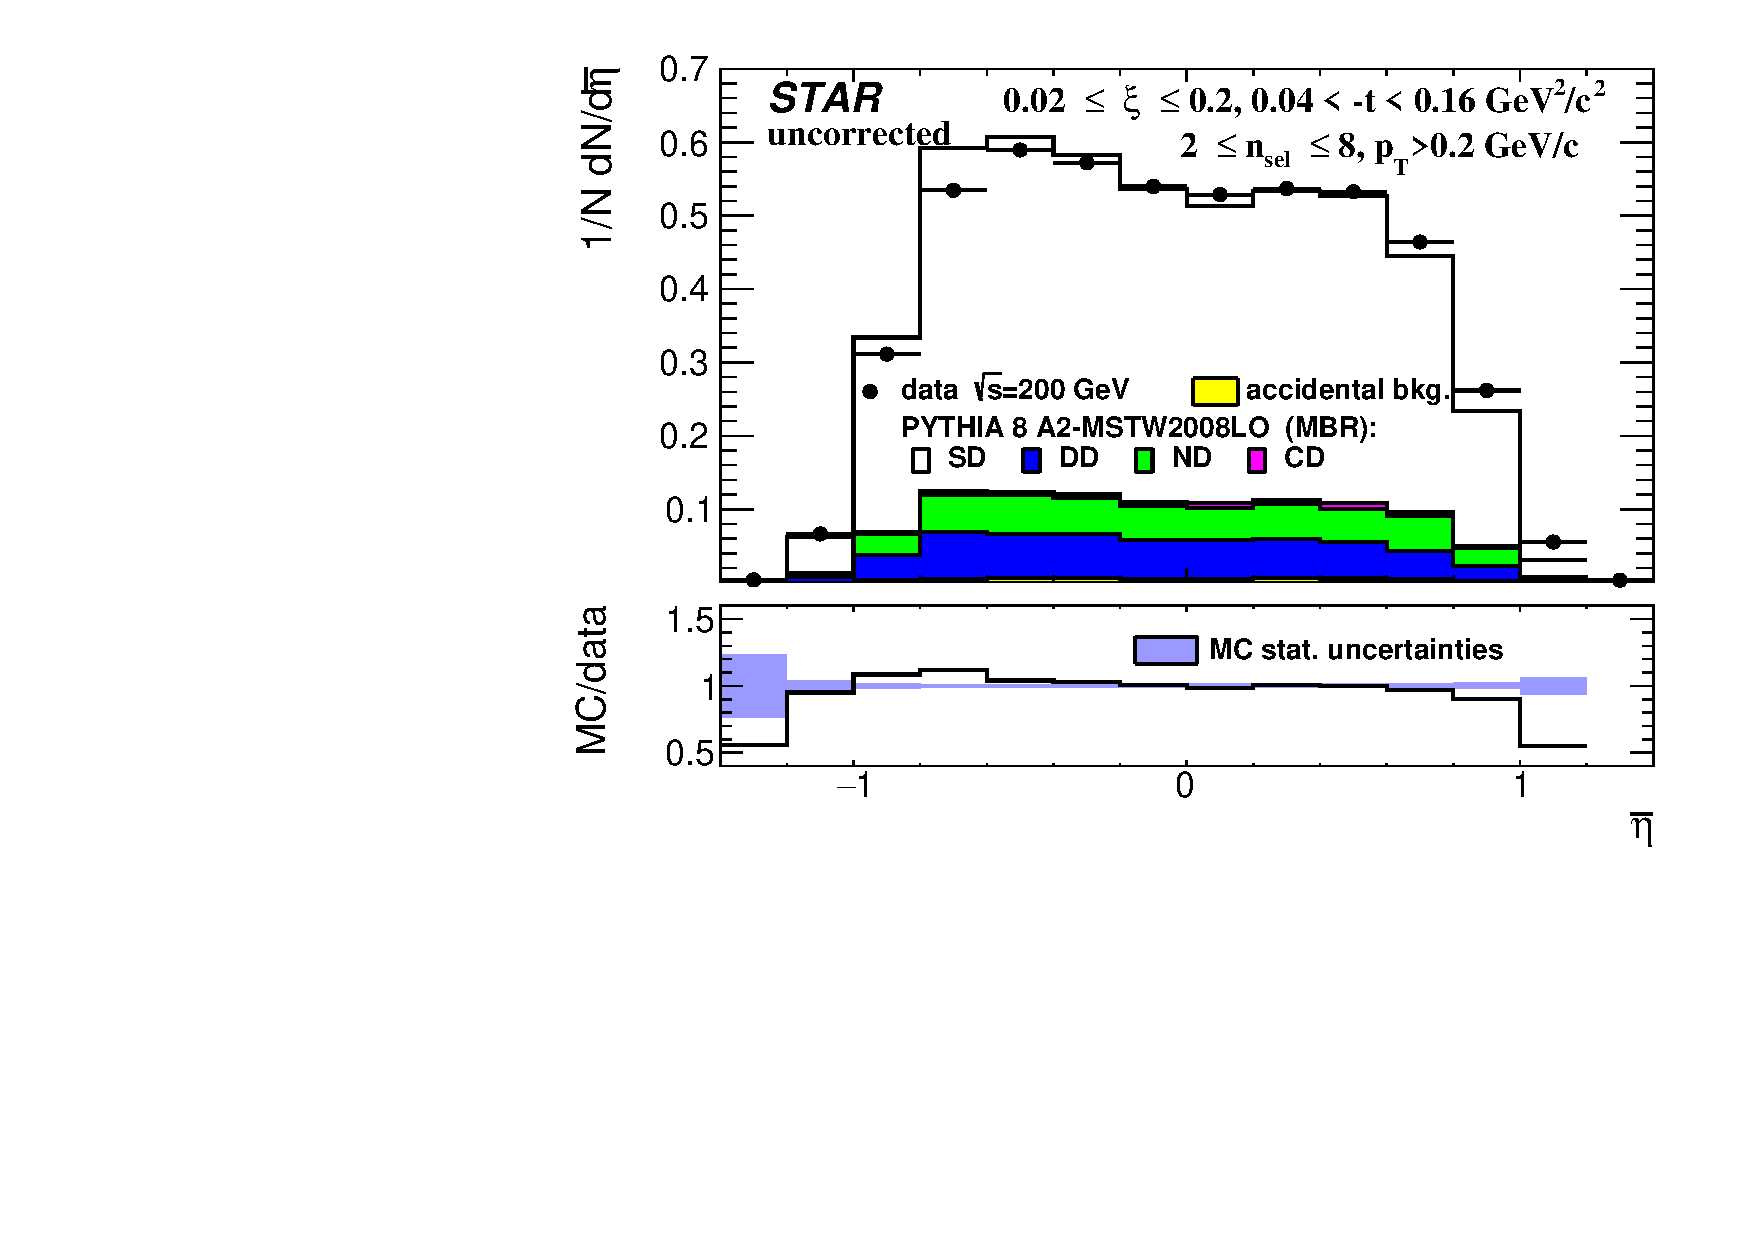
\includegraphics[width=\linewidth, page=1]{chapters/chrgSTAR/img/nonSD/chrg/SDT_pythia_xi0_RP_starsim_eta.pdf}
\end{subfigure}
\begin{subfigure}{.45\textwidth}
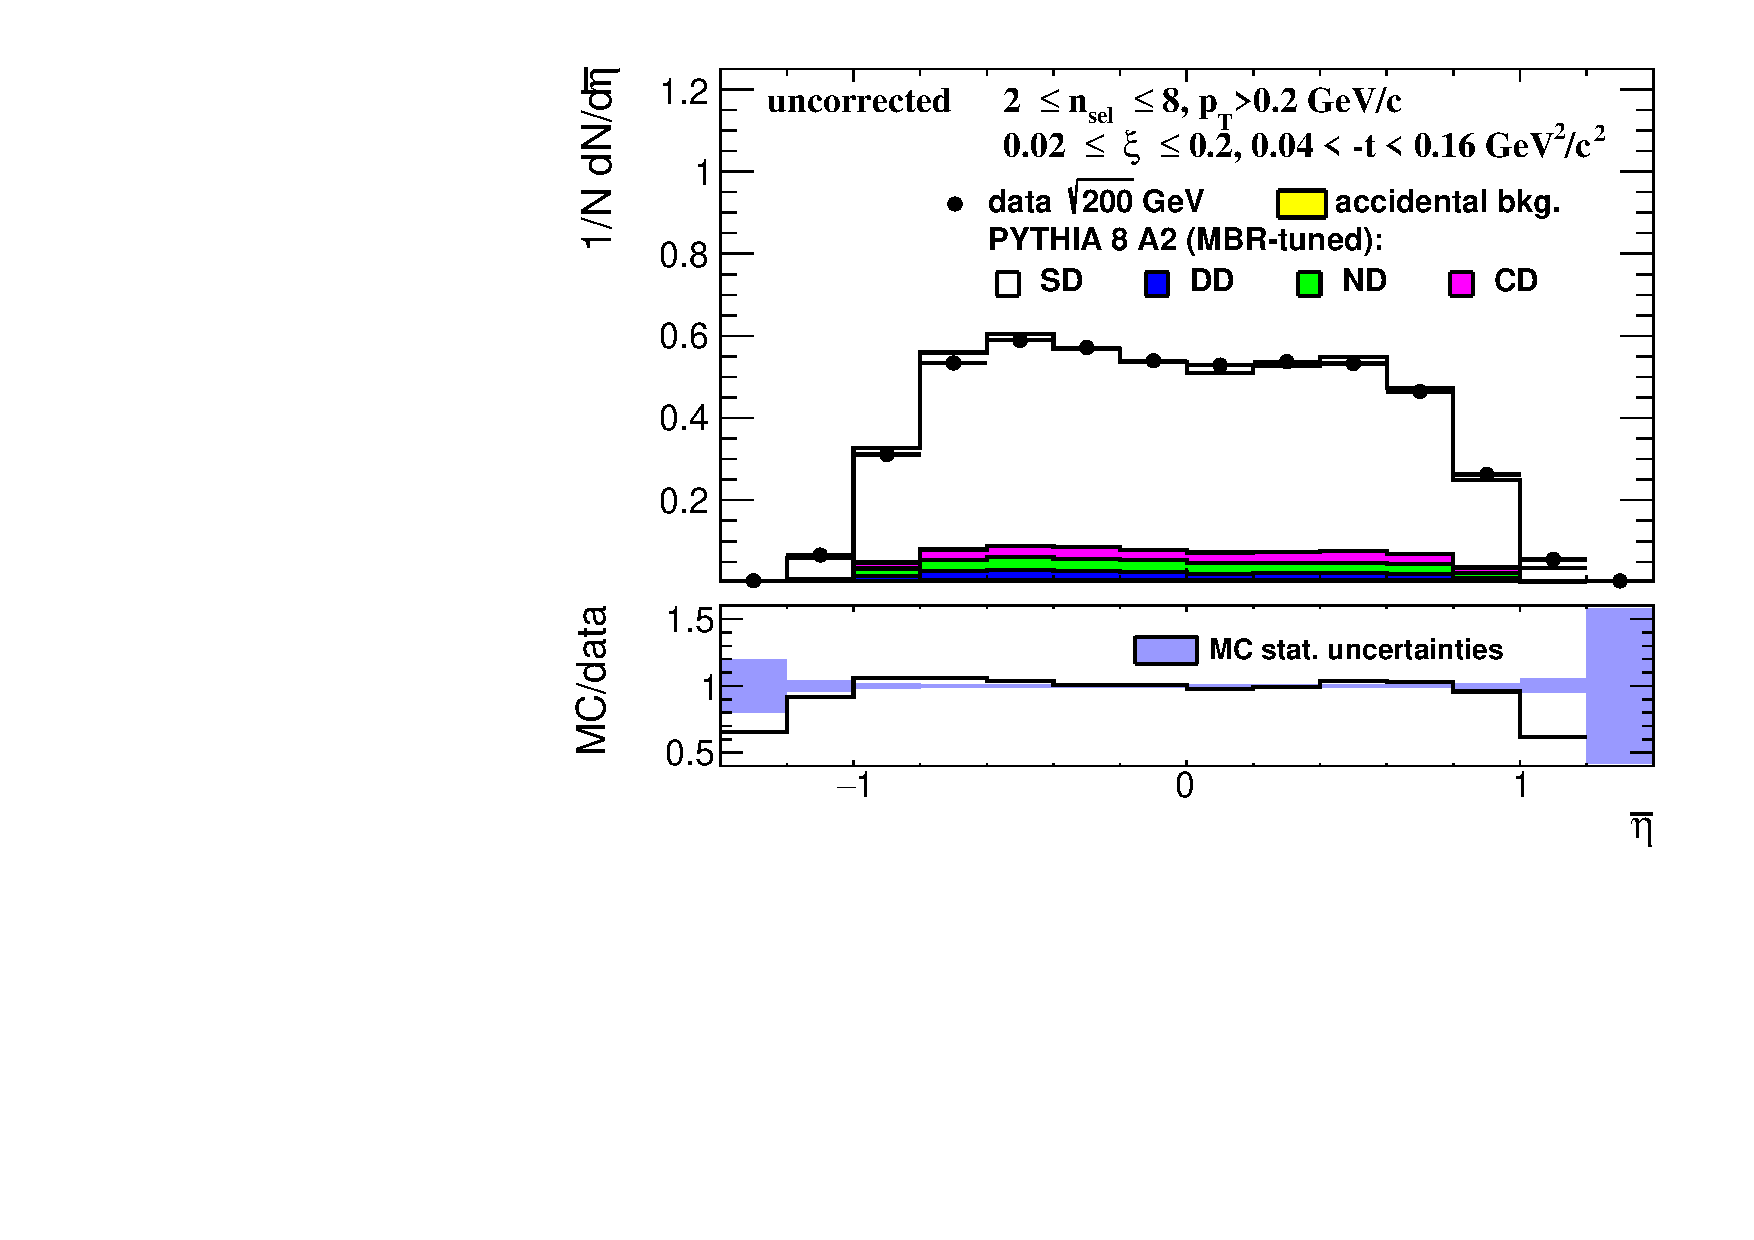
\includegraphics[width=\linewidth, page=1]{chapters/chrgSTAR/img/nonSD/chrg/SDT_pythia_xi0_option2_RP_starsim_eta.pdf}
\end{subfigure}
\begin{subfigure}{.45\textwidth}
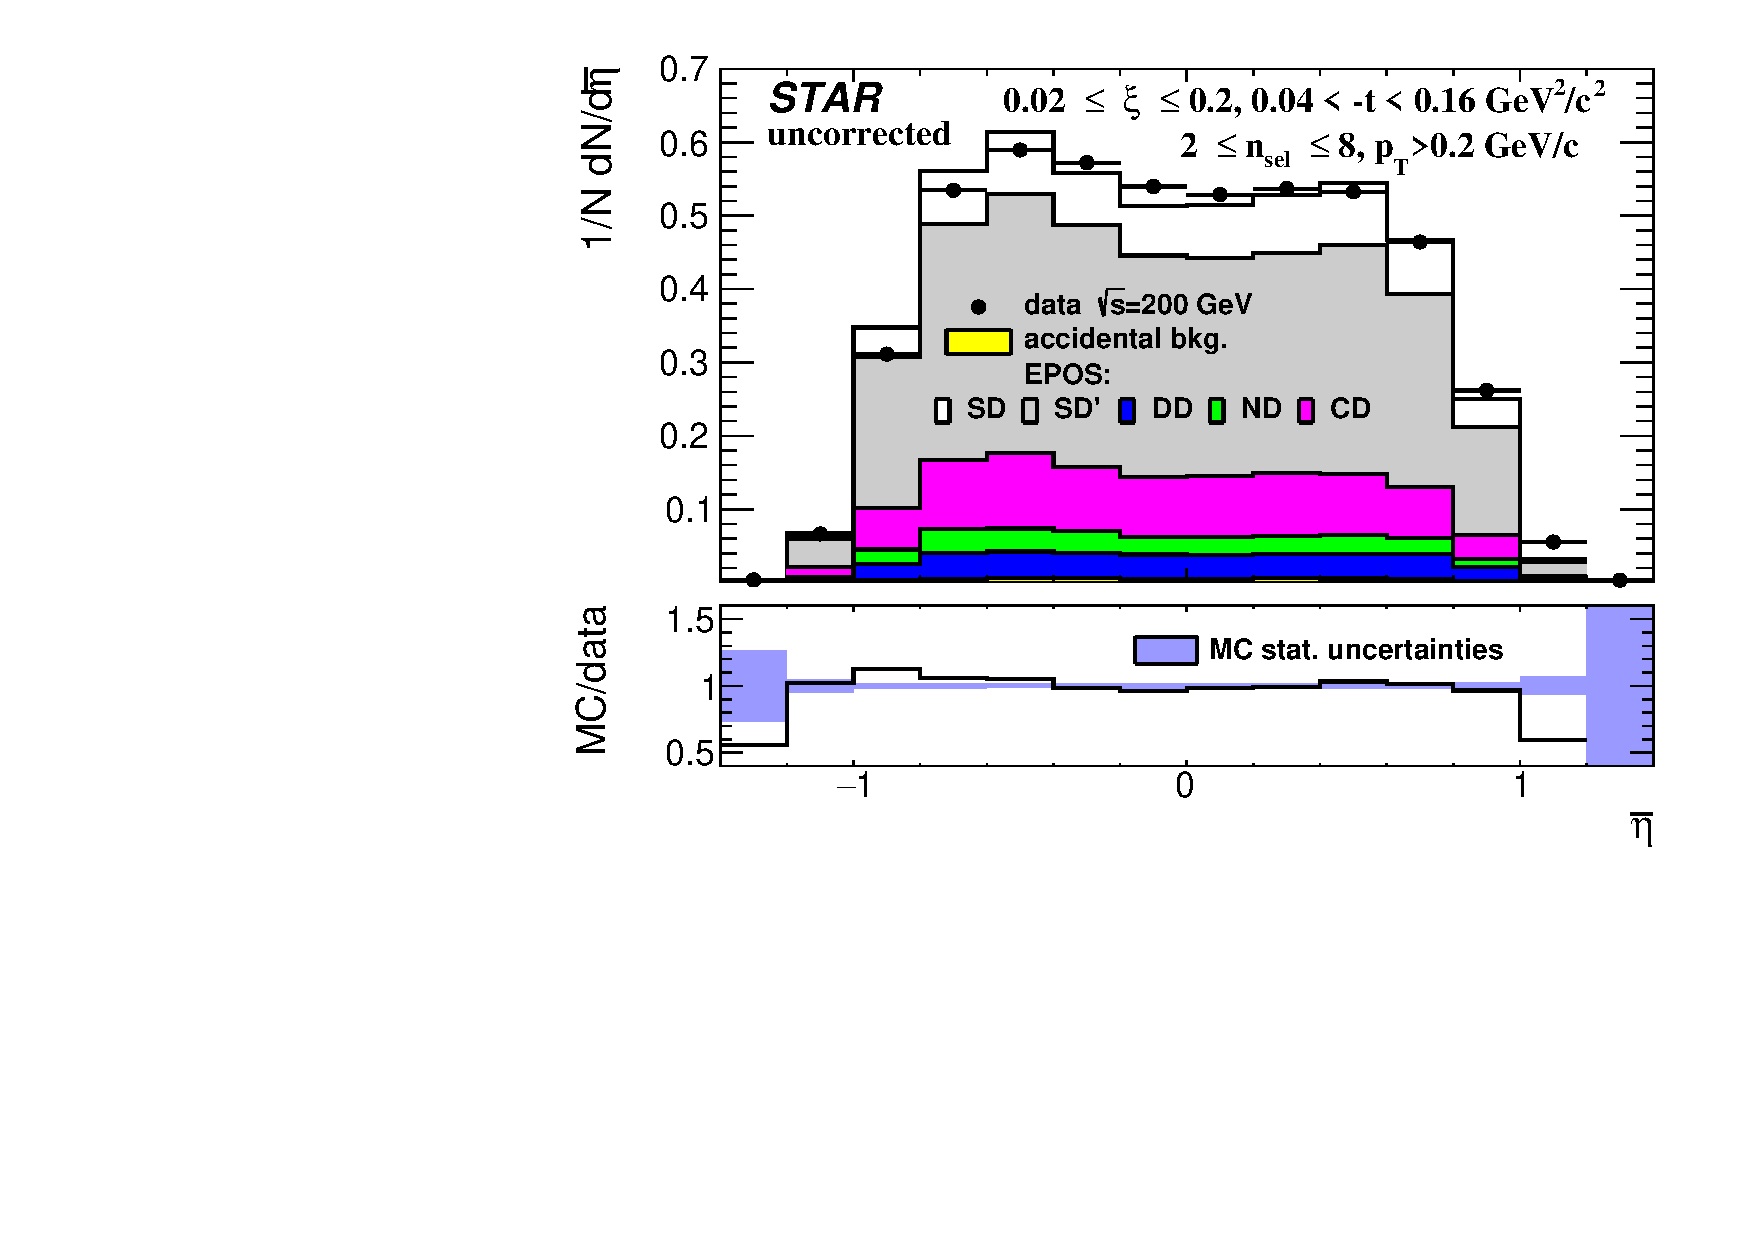
\includegraphics[width=\linewidth, page=1]{chapters/chrgSTAR/img/nonSD/chrg/SDT_epos_xi0_RP_starsim_eta.pdf}
\end{subfigure}
\begin{minipage}{.45\textwidth}
\caption{Uncorrected distributions of data compared to various MC models: (top left) PYTHIA8 A2 (MBR), (top right) PYTHIA8 A2 (MBR-tuned) and (bottom) EPOS, as a function of $\bar{\eta}$. }
\label{fig:nonSDera}
\end{minipage}

\end{figure}
\end{comment}
Events, in which  forward-scattered proton and reconstructed TOF
vertex are the result of the same $pp$ interaction, may originate from \ac{ND}, \ac{DD}, \ac{SD}, and \ac{CD} processes.  It is preferred to estimate the~background contribution from data, using dedicated control regions.
Since such regions were not found, the~relative contributions from the~above processes were  estimated from MC models and are therefore model dependent. Tracks reconstructed in \ac{RP}s  %which are modeled in the~\ac{MC} simulations are only coming from:
may also be:
\begin{itemize}
	\item forward-scattered protons produced in the \ac{SD}, \ac{CD} or \ac{DD} diffractive systems or from \ac{ND} events,
	\item secondary particles from showering initiated 
	by interaction of forward-scattered protons with beam-line elements. This contribution is negligible.
\end{itemize}


Figure~\ref{fig:nonSDxit} shows the uncorrected $\xi$ and $t$ distributions in data compared to various \ac{MC} models: PYTHIA~8 A2 (MBR), PYTHIA~8 A2 (MBR-tuned), PYTHIA~8 4C (SaS) and EPOS. The \ac{MC} distributions are split into \ac{SD}, \ac{ND}, \ac{DD} and \ac{CD} components. For EPOS, SD$^\prime$ is separated from the ND events. Additionally, the accidental background is also shown. PYTHIA~8 A2 (MBR) predictions, shown in Fig.~\ref{fig:nonSDxit} (a-b), do not agree with the data, especially  there is small number of events in the~region of large values of $\xi$. 
This effect may be due to the~scaling factors, which are introduced in PYTHIA~8 to artificially suppress diffractive cross sections in the~high mass region, or due to too large Pomeron intercept ($\epsilon=0.104$).
 Therefore,
additional two samples of PYTHIA~8 were generated: without this artificial suppression  (\mbox{MBR-tuned}) and with  $\epsilon=0$ (\mbox{SaS}). Their predictions, shown in Fig.~\ref{fig:nonSDxit} (c-f), agree much better with the~data than PYTHIA~8 A2 (MBR) and result also in a~suppression of non-SD events. Amongst PYTHIA~8 models, PYTHIA~8 A2 (MBR-tuned) shows the~best agreement  with the~data.
EPOS predictions,  shown in Fig.~\ref{fig:nonSDxit} (g-h), describes data better than PYTHIA~8 but shows a dominant contribution of SD$^\prime$ events. The~CD contribution in EPOS is several times greater than in PYTHIA~8 (MBR), but it was never tuned to describe any data, as opposed to PYTHIA~8 (MBR) in which the~\ac{CD} cross sections are constrained by CDF measurements~\cite{Acosta:2003xi}. 
The~\ac{CD} component in the~\ac{SaS} model is based on simple scaling assumption, therefore, it is not usually used by the~experimental communities. All MCs predict significant \ac{DD} and \ac{ND} background at large $\xi$, thereby  the analysis was limited to $\xi < 0.2$. 


\Cref{fig:nonSDnsel,fig:nonSDpt,fig:nonSDera} show the uncorrected distributions of variables used in the later analysis: $n_{\mathrm{sel}}$, $p_{\mathrm T}$ an $\bar{\eta}$. The  contributions from non-SD (except  EPOS SD$^\prime$) interactions differ a bit between each other, i.e. EPOS predicts significantly larger CD contribution, whereas DD and ND are suppressed in PYTHIA~8 A2 (MBR-tuned) and PYTHIA~8 4C (SaS).  PYTHIA~8~A2~(MBR) is used as the default model  of non-SD contribution subtracted from the data with systematic uncertainty $\pm50\%$, which covers all differences between the~models except EPOS SD$^\prime$.  In this analysis EPOS SD$^\prime$ is   considered as an~alternative to PYTHIA~8 SD model of events with forward-scattered proton in the final state,  where one of the proton remnants hadronizes back to a~single proton (non-diffractive process), while in  PYTHIA~8 the~initial proton stays intact (diffractive process). As a~consequence, results  are compared  with the~sum of SD and SD$^\prime$ processes for EPOS model.  
%\end{comment}
%\thispagestyle{empty}

%\newpage
\begin{figure}[H]
	%\vspace{-1.cm}
	\thisfloatpagestyle{fancy}
	\centering
	\begin{overpic}[width=0.47\textwidth,tics=4,page=1]{chapters/chrgSTAR/img/nonSD/SDT_pythia_xi0_RP_starsim_xi.pdf}
		\put (88,40) {\Large{a}}
	\end{overpic}
	\vspace{-0.2cm}
	\begin{overpic}[width=0.47\textwidth,tics=4,page=1]{chapters/chrgSTAR/img/nonSD/SDT_pythia_xi0_RP_starsim_t.pdf}
		\put (85,35) {\Large{b}}
	\end{overpic}
	\begin{overpic}[width=0.47\textwidth,tics=4,page=1]{chapters/chrgSTAR/img/nonSD/SDT_pythia_xi0_option2_RP_starsim_xi.pdf}
		\put (85,35) {\Large{c}}
	\end{overpic}
	\vspace{-0.2cm}
	\begin{overpic}[width=0.47\textwidth,tics=4,page=1]{chapters/chrgSTAR/img/nonSD/SDT_pythia_xi0_option2_RP_starsim_t.pdf}
		\put (85,35) {\Large{d}}
	\end{overpic}
	\begin{overpic}[width=0.47\textwidth,tics=4,page=1]{chapters/chrgSTAR/img/nonSD/SDT_pythia_xi0_sas_RP_starsim_xi.pdf}
		\put (85,35) {\Large{e}}
	\end{overpic}
	\vspace{-0.2cm}
	\begin{overpic}[width=0.47\textwidth,tics=4,page=1]{chapters/chrgSTAR/img/nonSD/SDT_pythia_xi0_sas_RP_starsim_t.pdf}
		\put (85,35) {\Large{f}}
	\end{overpic}
	\begin{overpic}[width=0.47\textwidth,tics=4,page=1]{chapters/chrgSTAR/img/nonSD/SDT_epos_xi0_RP_starsim_xi.pdf}
		\put (85,35) {\Large{g}}
	\end{overpic}
	\vspace{-0.2cm}
	\begin{overpic}[width=0.47\textwidth,tics=4,page=1]{chapters/chrgSTAR/img/nonSD/SDT_epos_xi0_RP_starsim_t.pdf}
		\put (85,35) {\Large{h}}
	\end{overpic}
	\vspace{-0.2cm}
	%
	\caption{Uncorrected distributions of data compared to various MC models: (a-b) PYTHIA~8 A2 (MBR), (c-d) PYTHIA~8 A2 (MBR-tuned), (e-f) PYTHIA~8 4C (SaS) and (g-h) EPOS, as a~function of (left column) $\xi$  and (right column) $|t|$. The~ratio of MC predictions and data is shown in the~bottom panels.}
	\label{fig:nonSDxit}
	%\vspace{-0.5cm}
\end{figure}

\begin{figure}[t!]
	\vspace{-1.5cm}
	\thisfloatpagestyle{fancy}
	\centering
	\begin{subfigure}{.49\textwidth}
		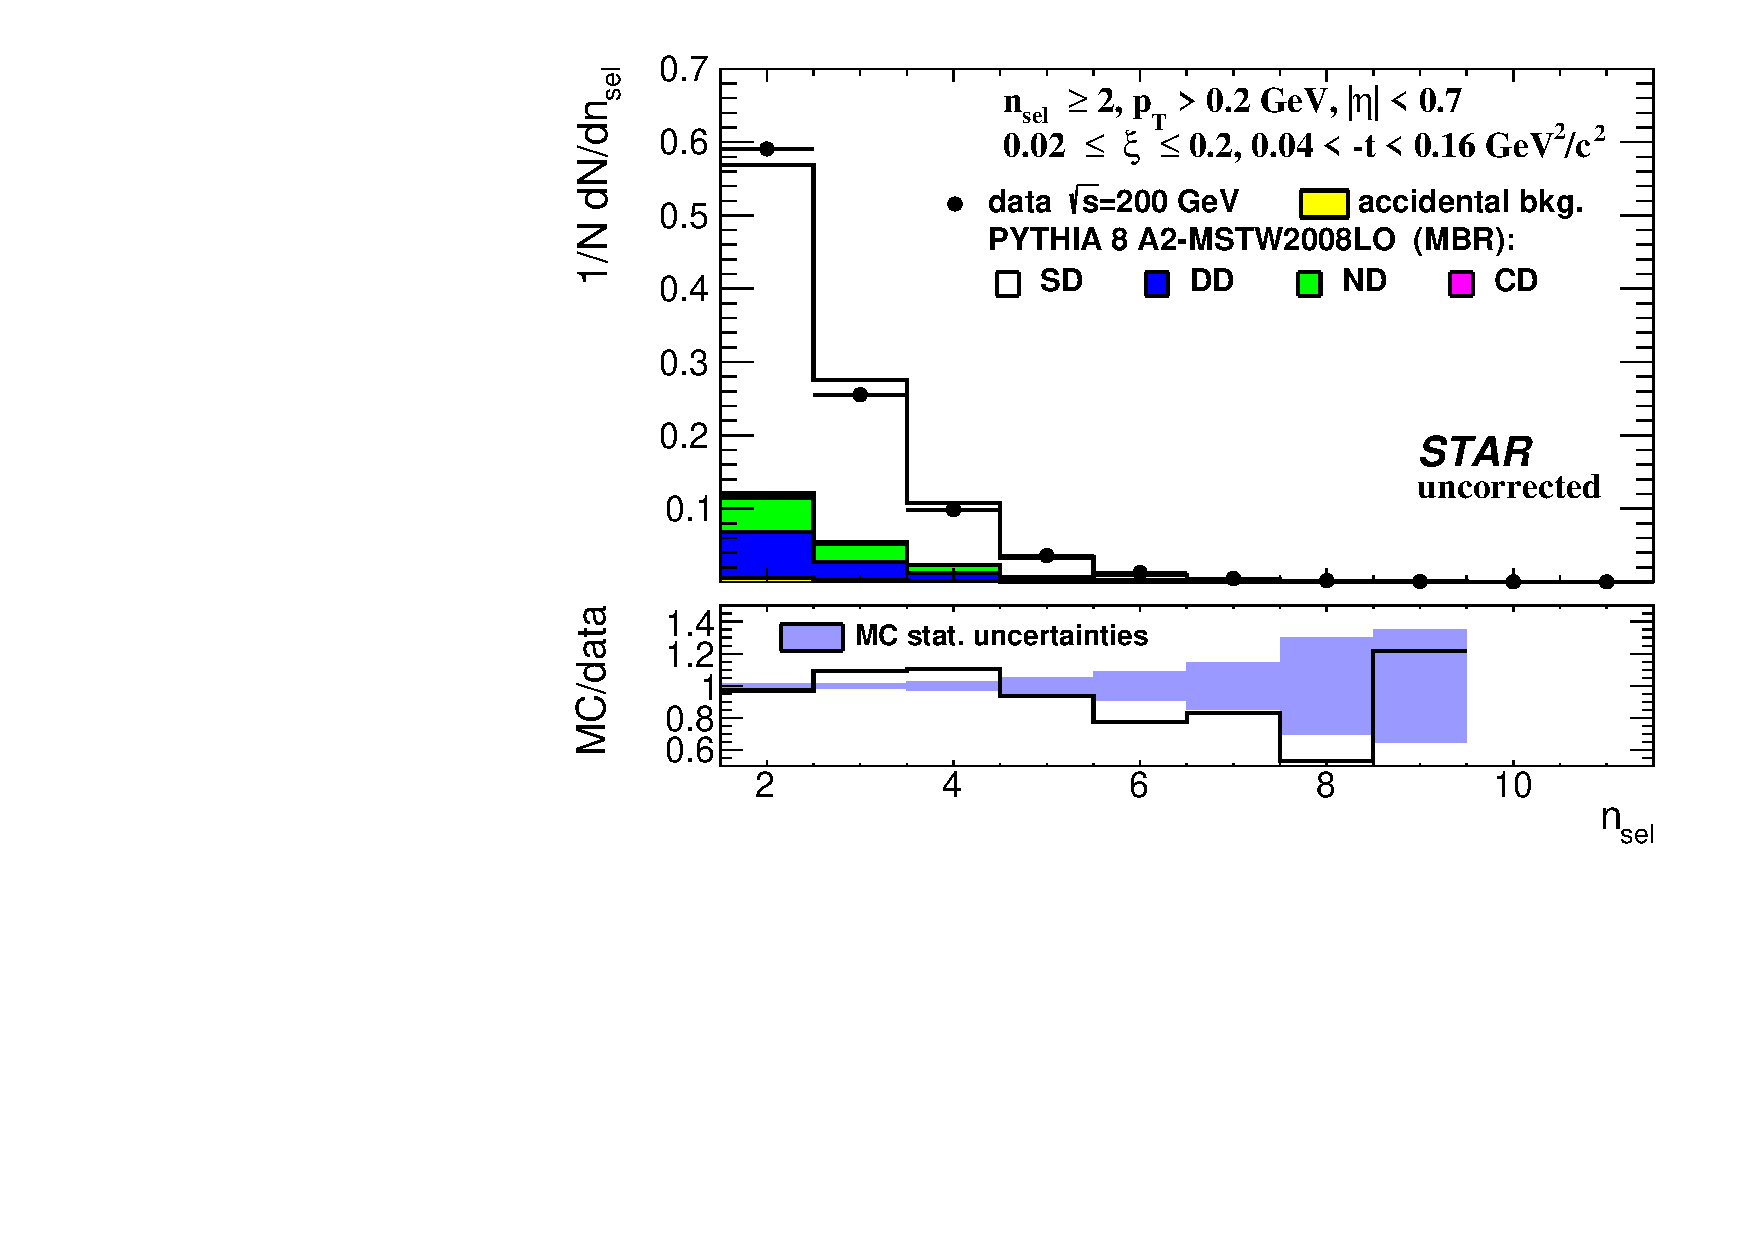
\includegraphics[width=\linewidth, page=1]{chapters/chrgSTAR/img/nonSD/chrg/SDT_pythia_xi0_RP_starsim_nsel.pdf}
	\end{subfigure}
	\begin{subfigure}{.49\textwidth}
		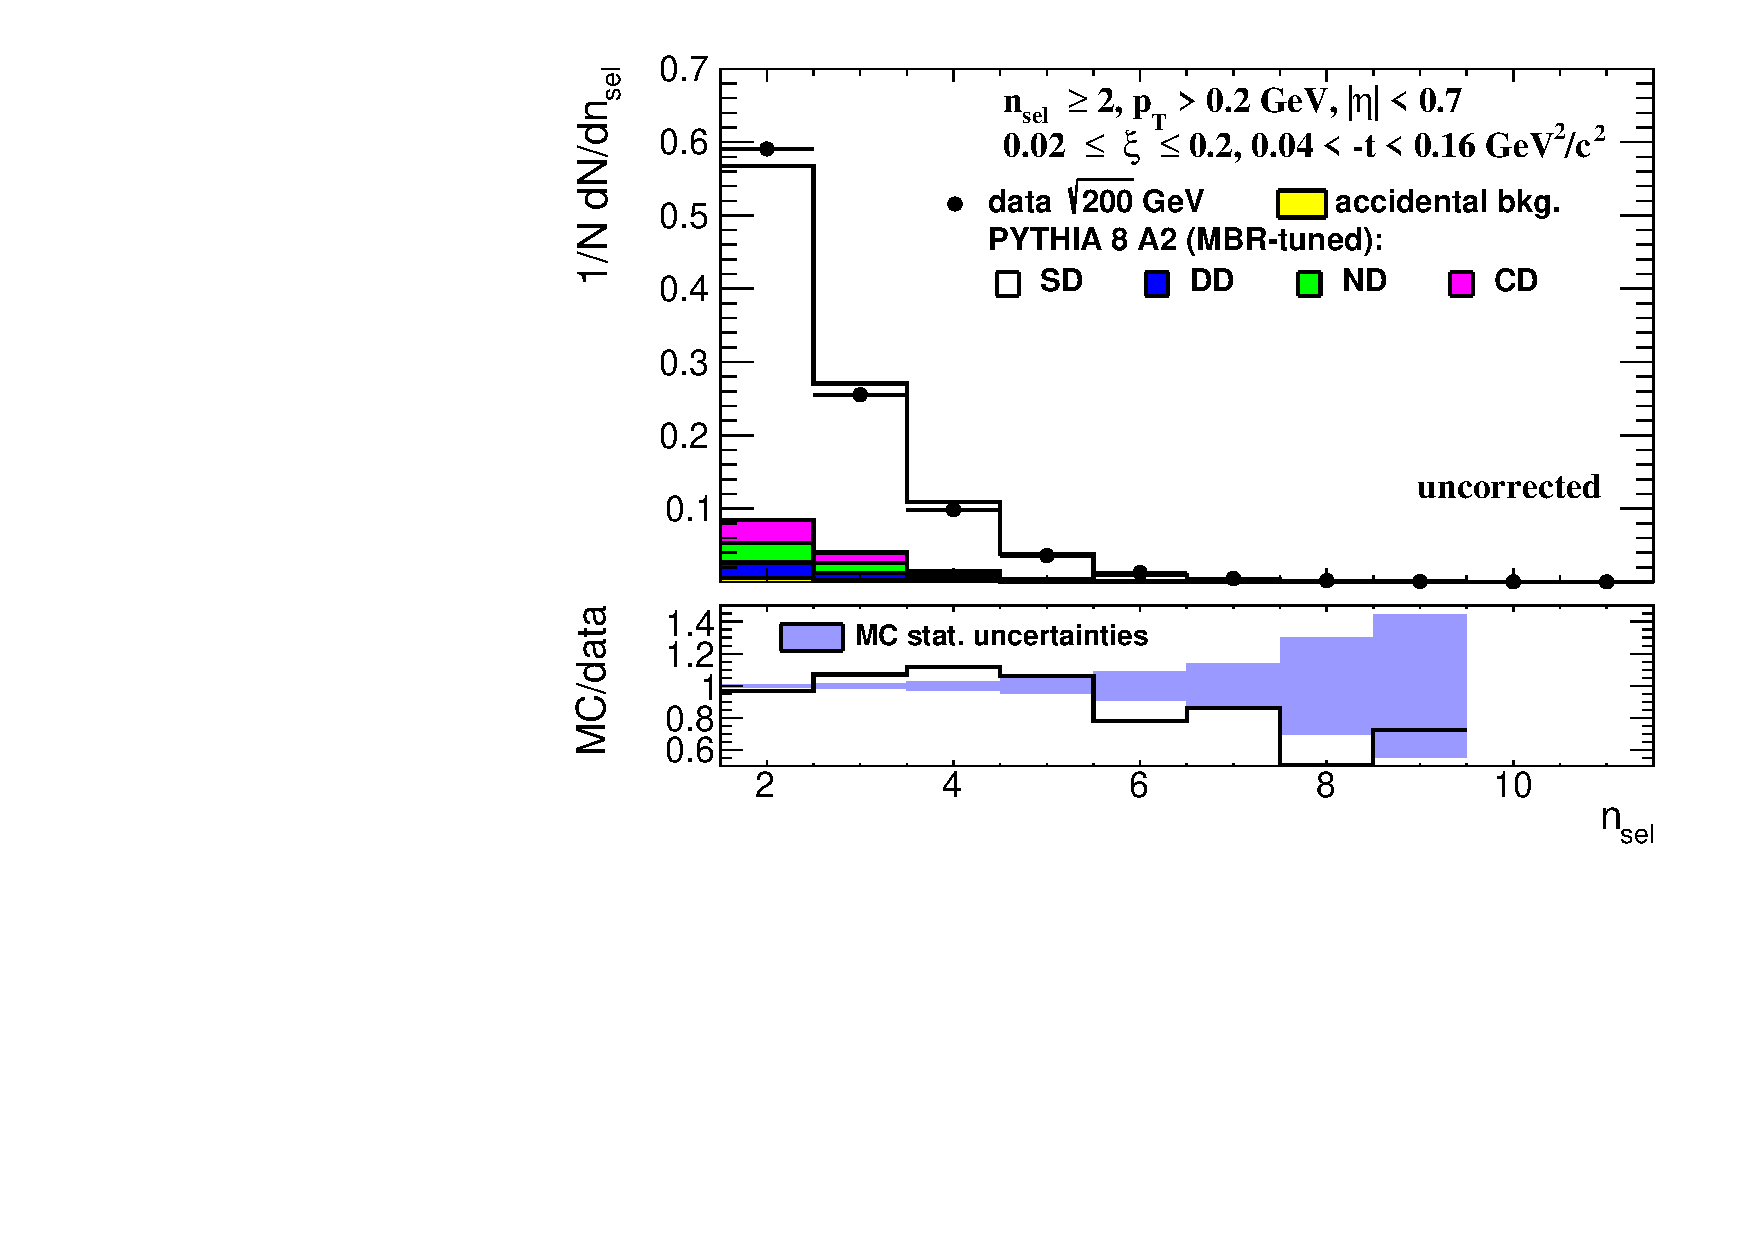
\includegraphics[width=\linewidth, page=1]{chapters/chrgSTAR/img/nonSD/chrg/SDT_pythia_xi0_option2_RP_starsim_nsel.pdf}
	\end{subfigure}
	\begin{subfigure}{.49\textwidth}
		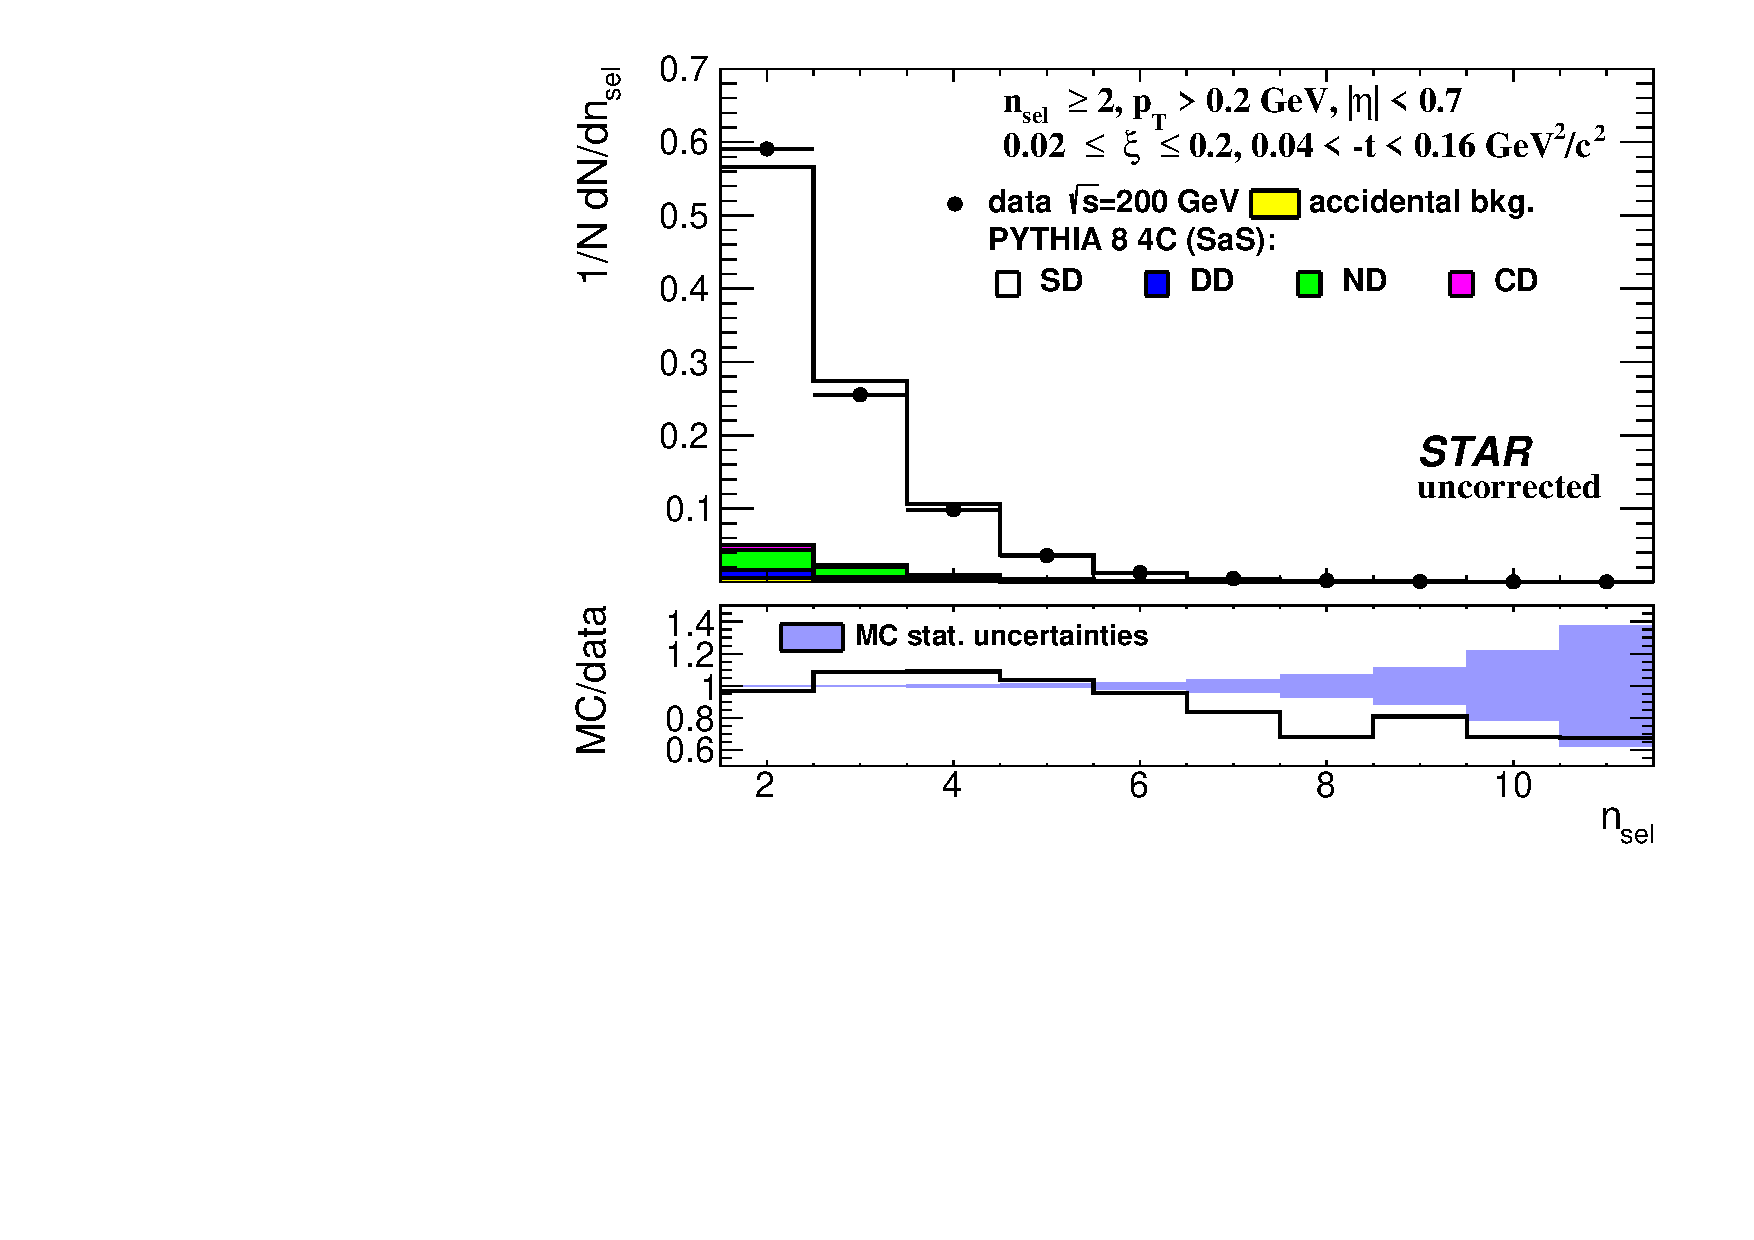
\includegraphics[width=\linewidth, page=1]{chapters/chrgSTAR/img/nonSD/SDT_pythia_xi0_sas_RP_starsim_nsel.pdf}
	\end{subfigure}
	\begin{subfigure}{.49\textwidth}
		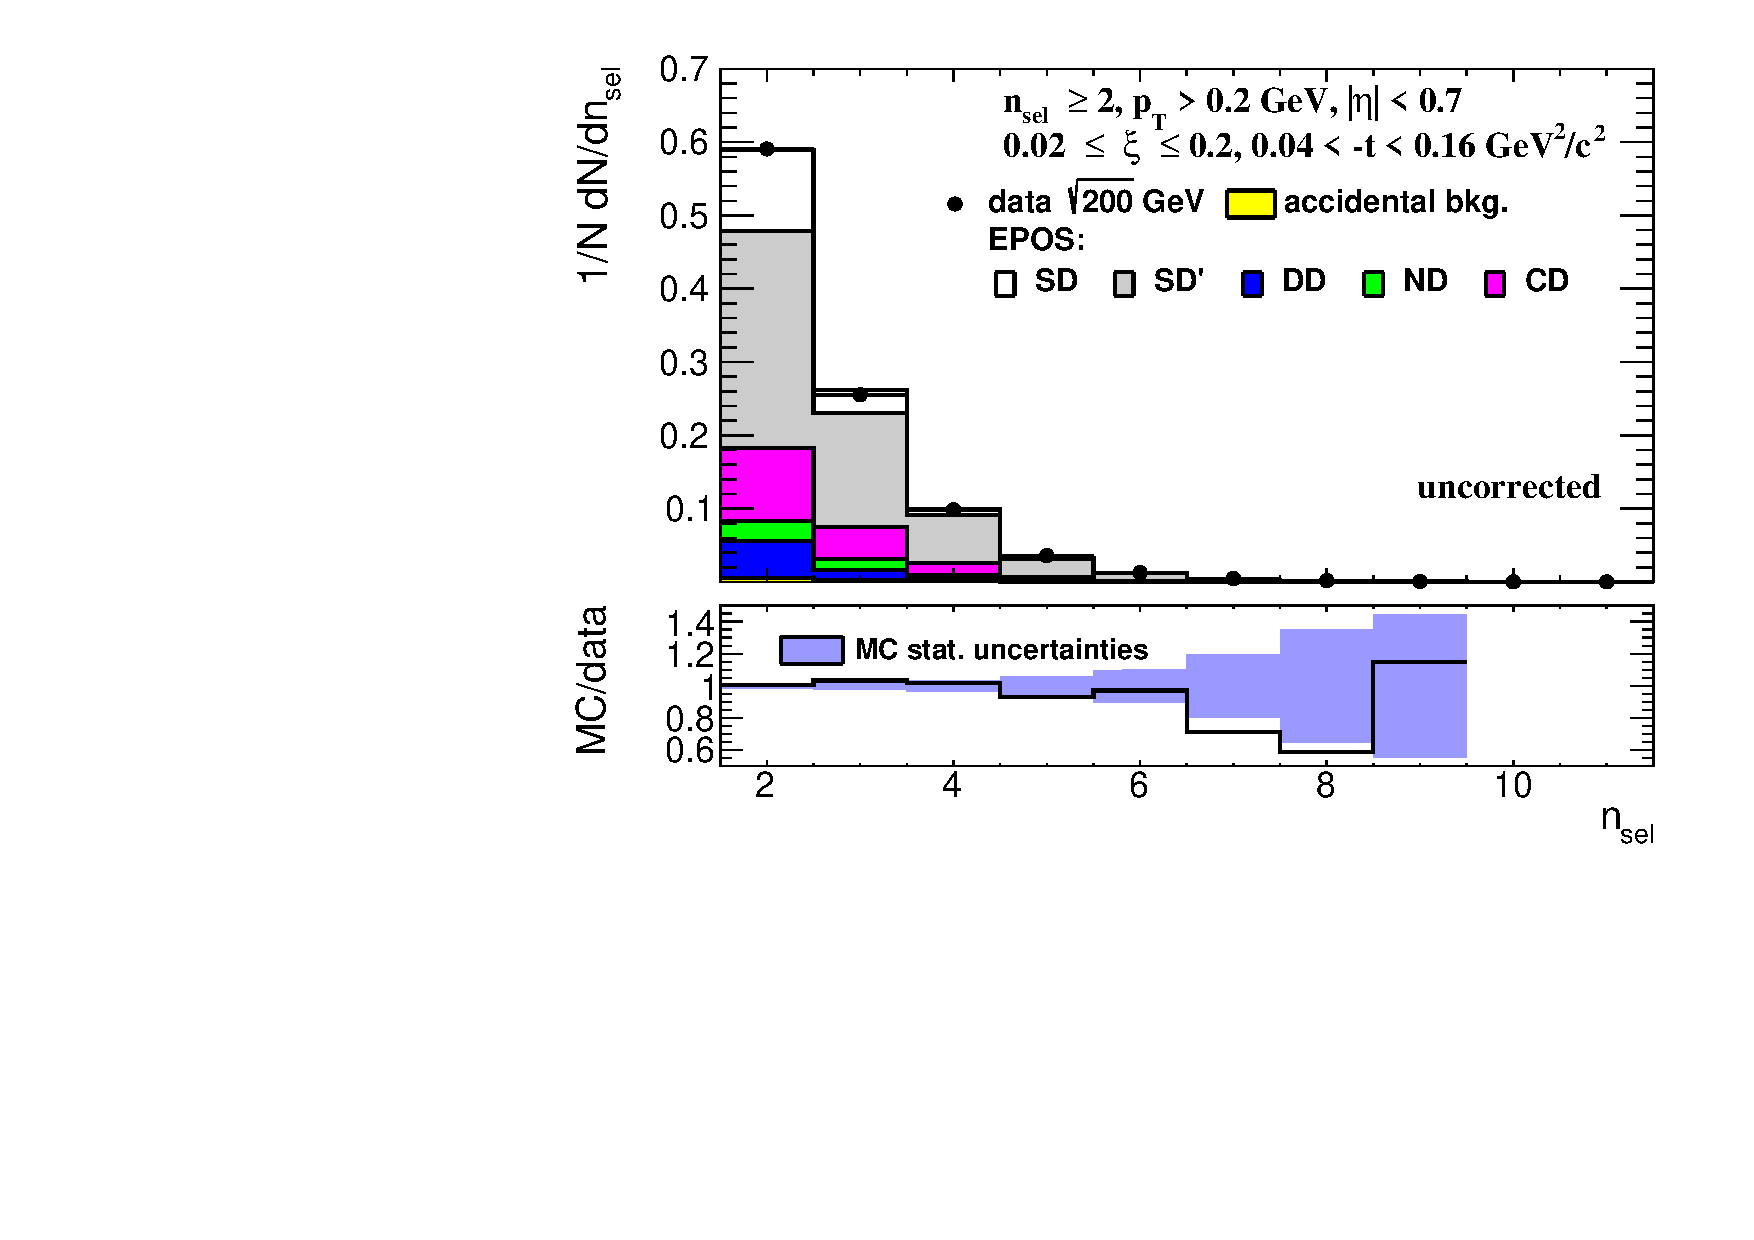
\includegraphics[width=\linewidth, page=1]{chapters/chrgSTAR/img/nonSD/chrg/SDT_epos_xi0_RP_starsim_nsel.pdf}
	\end{subfigure}
	%\begin{minipage}{.49\textwidth}
	\caption{Uncorrected distributions of data compared to various MC models: (top left) PYTHIA~8 A2 (MBR), (top right) PYTHIA~8 A2 (MBR-tuned), (bottom left) PYTHIA~8 4C (SaS) and (bottom right) EPOS, as a function of $n_{\mathrm{sel}}$. The~ratio of MC predictions and data is shown in the~bottom panels.}
	\label{fig:nonSDnsel}
	%\end{minipage}
	
%\end{figure}

%\begin{figure}[t!]
	%\vspace{-0.5cm}
	\centering
	\begin{subfigure}{.49\textwidth}
		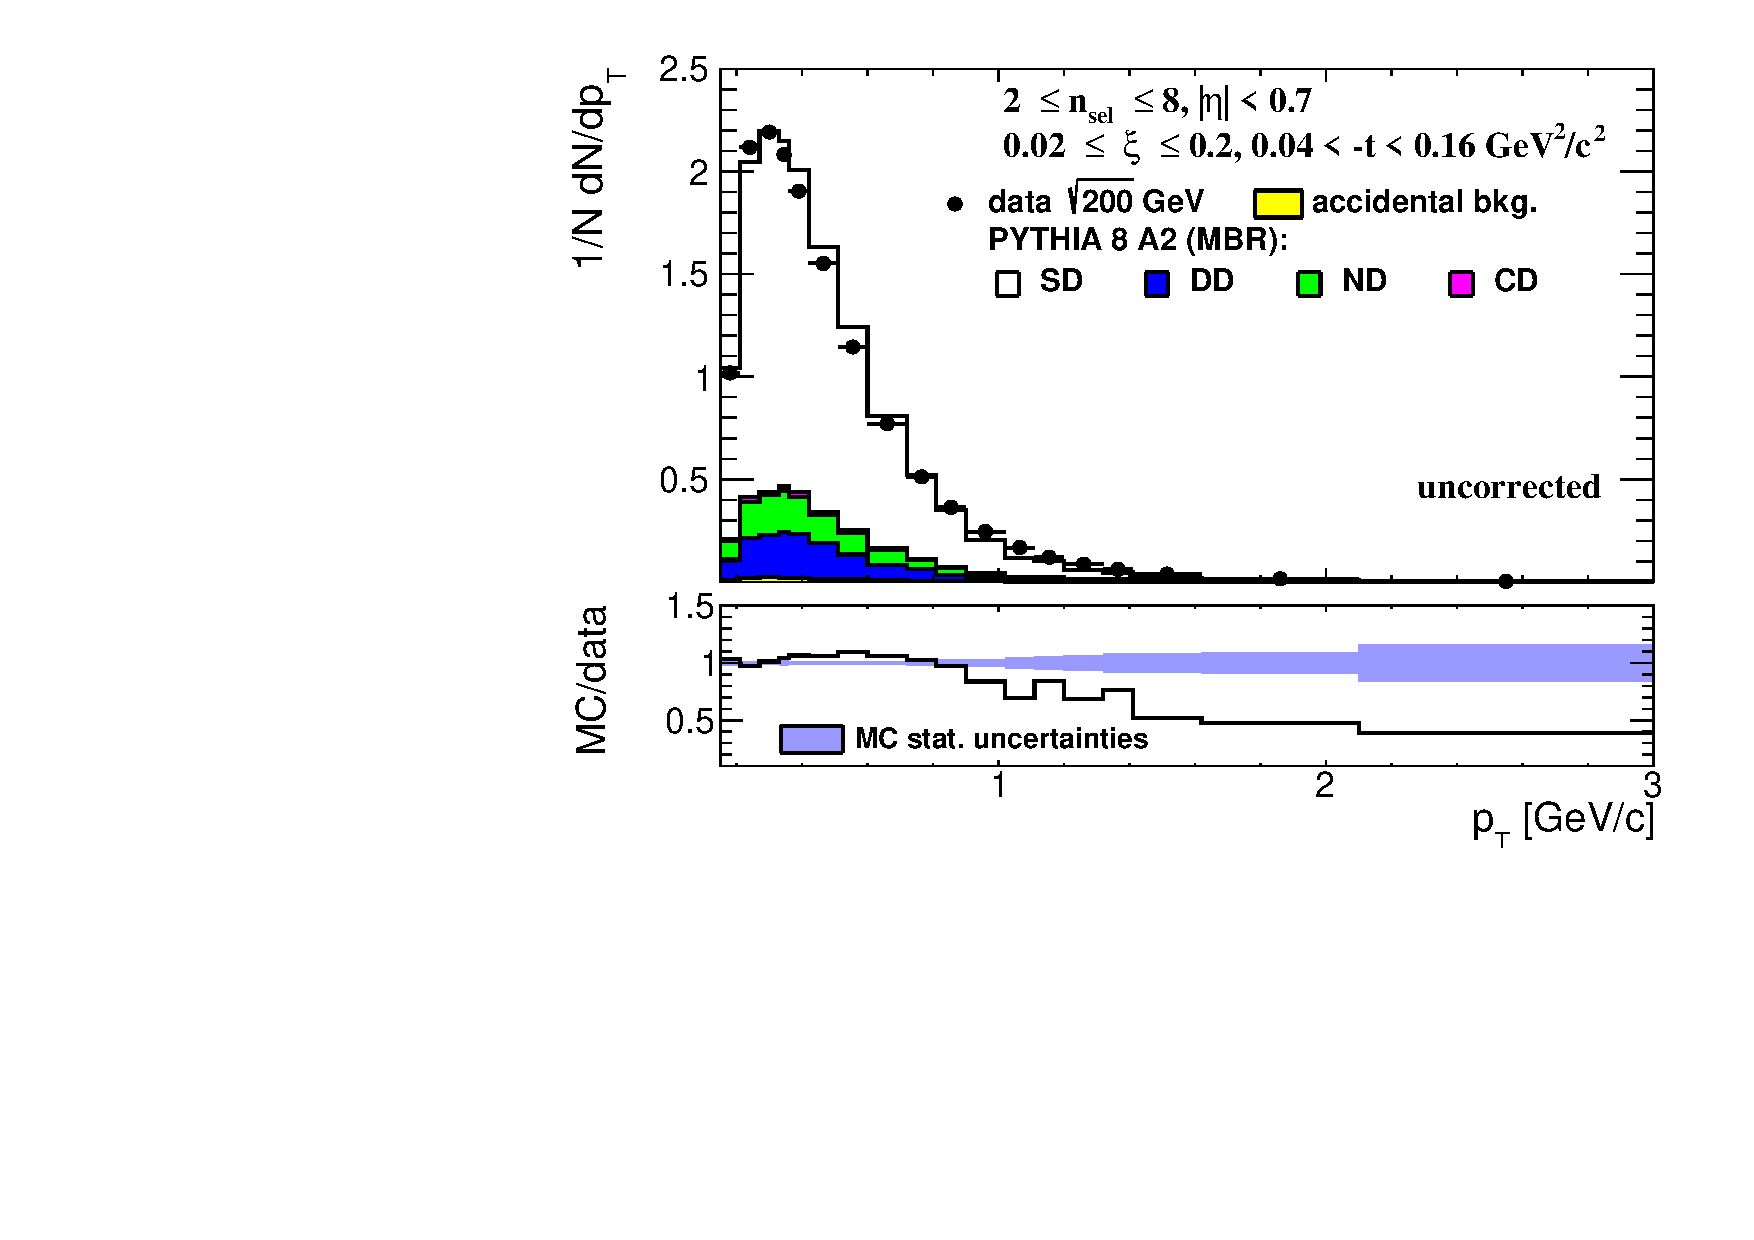
\includegraphics[width=\linewidth, page=1]{chapters/chrgSTAR/img/nonSD/chrg/SDT_pythia_xi0_RP_starsim_pt.pdf}
	\end{subfigure}
	\begin{subfigure}{.49\textwidth}
		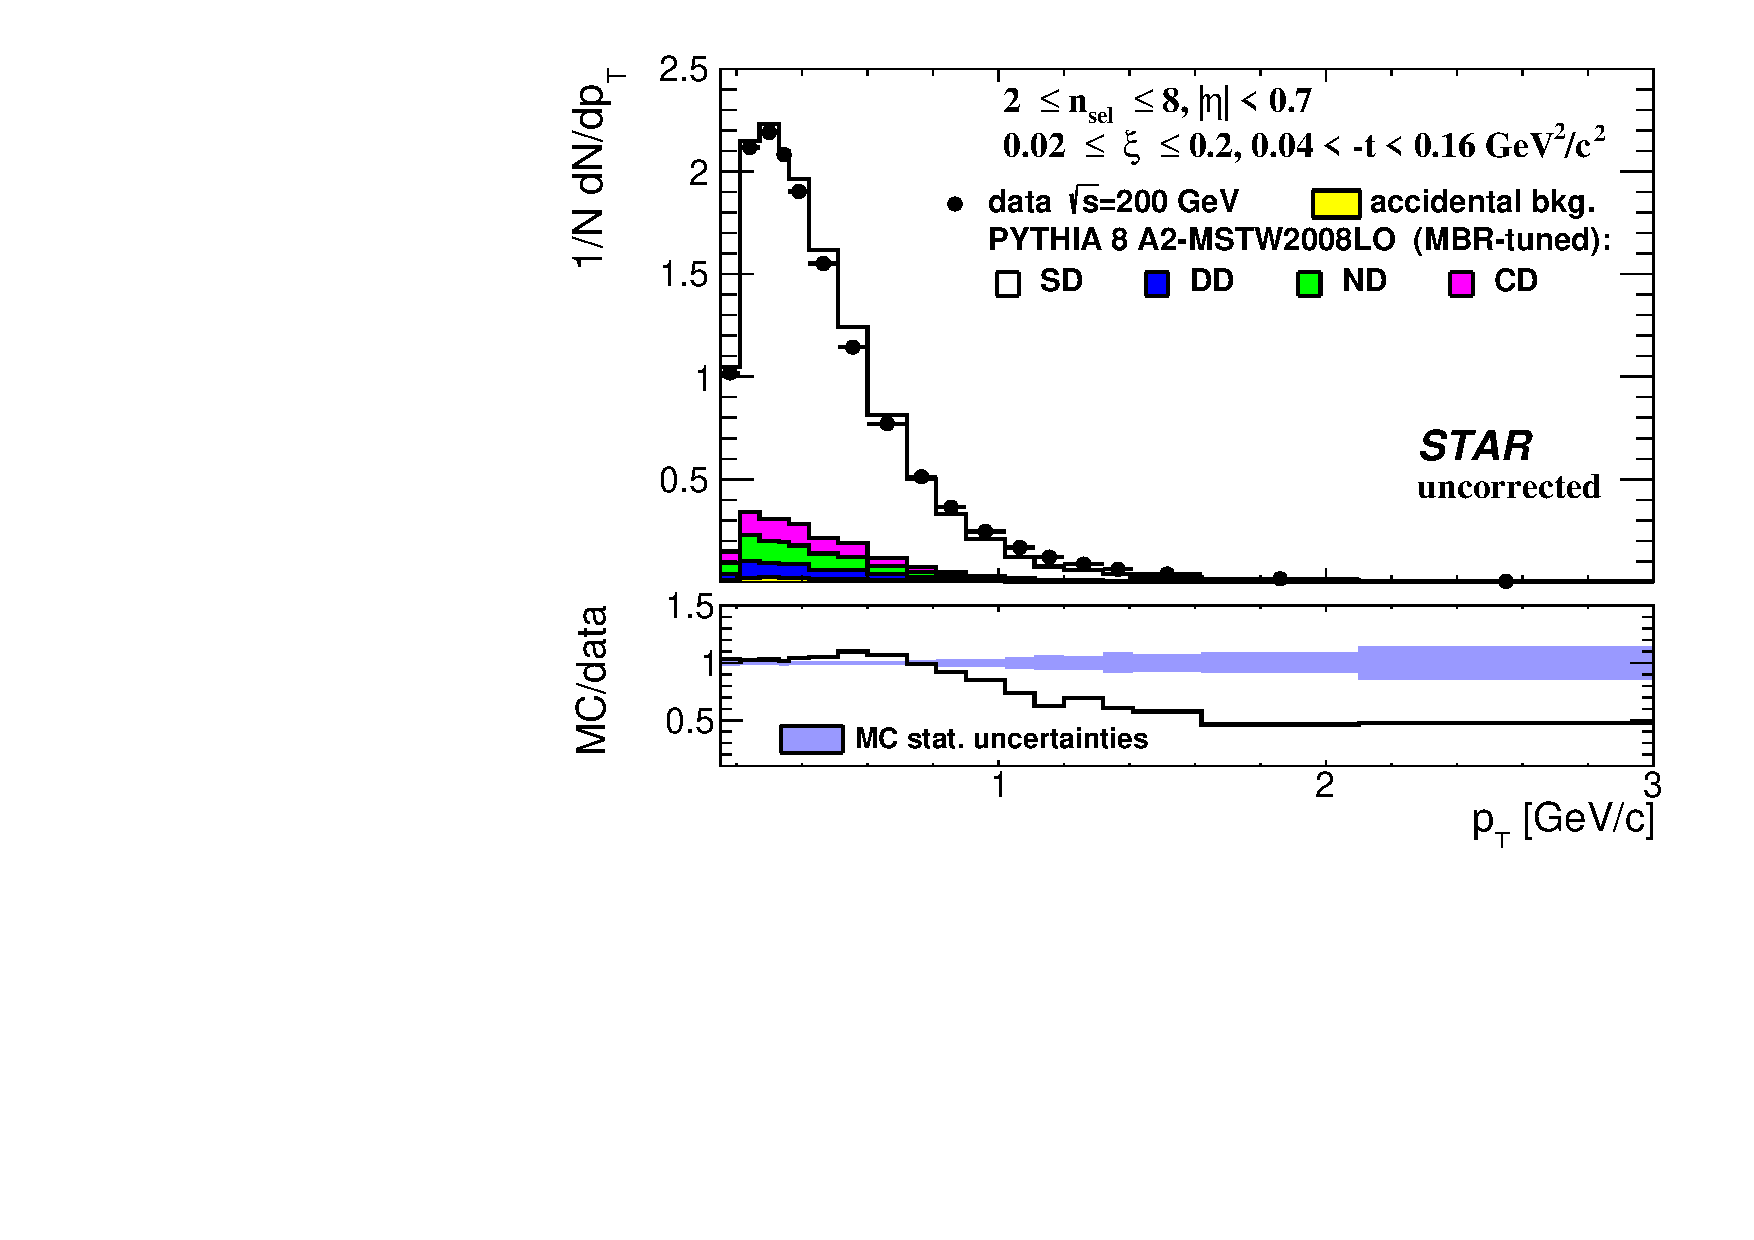
\includegraphics[width=\linewidth, page=1]{chapters/chrgSTAR/img/nonSD/chrg/SDT_pythia_xi0_option2_RP_starsim_pt.pdf}
	\end{subfigure}
	\begin{subfigure}{.49\textwidth}
		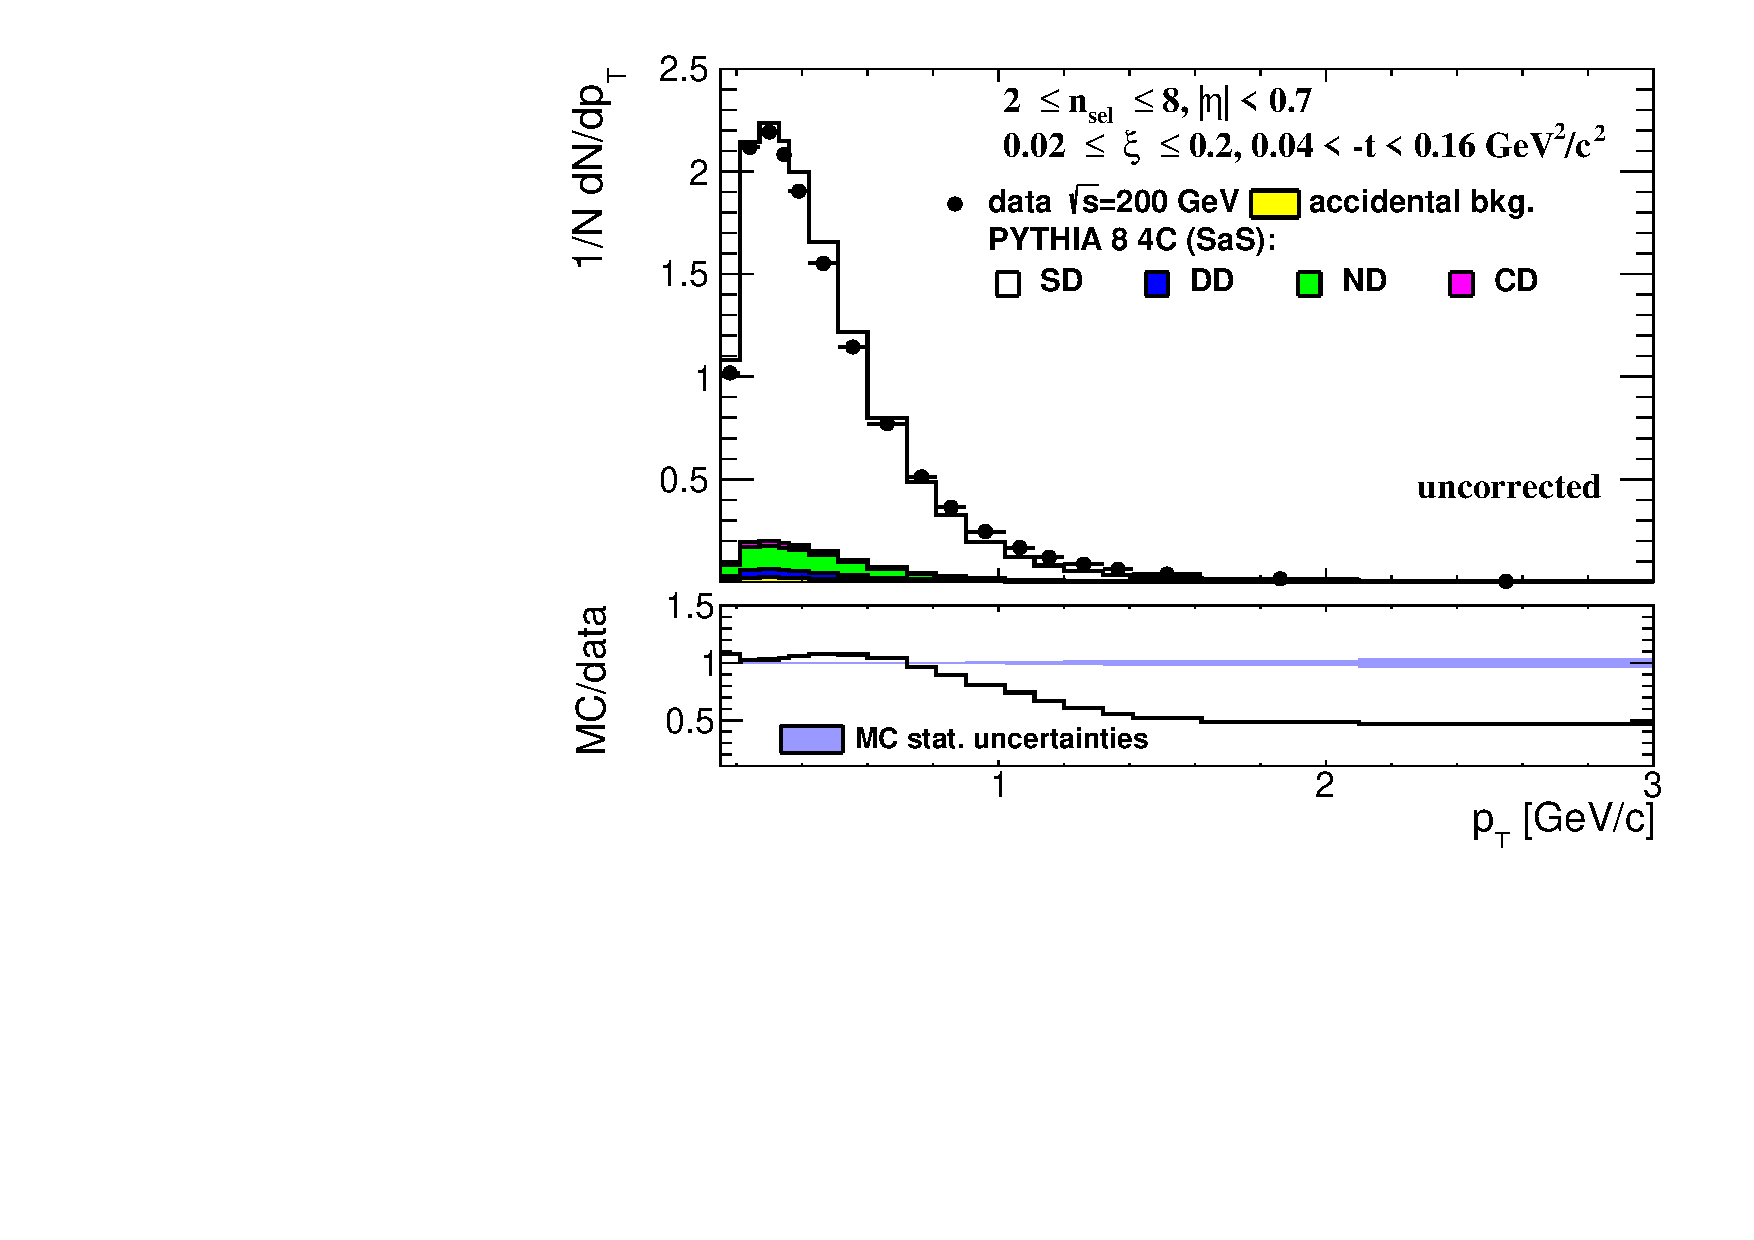
\includegraphics[width=\linewidth, page=1]{chapters/chrgSTAR/img/nonSD/SDT_pythia_xi0_sas_RP_starsim_pt.pdf}
	\end{subfigure}
	\begin{subfigure}{.49\textwidth}
		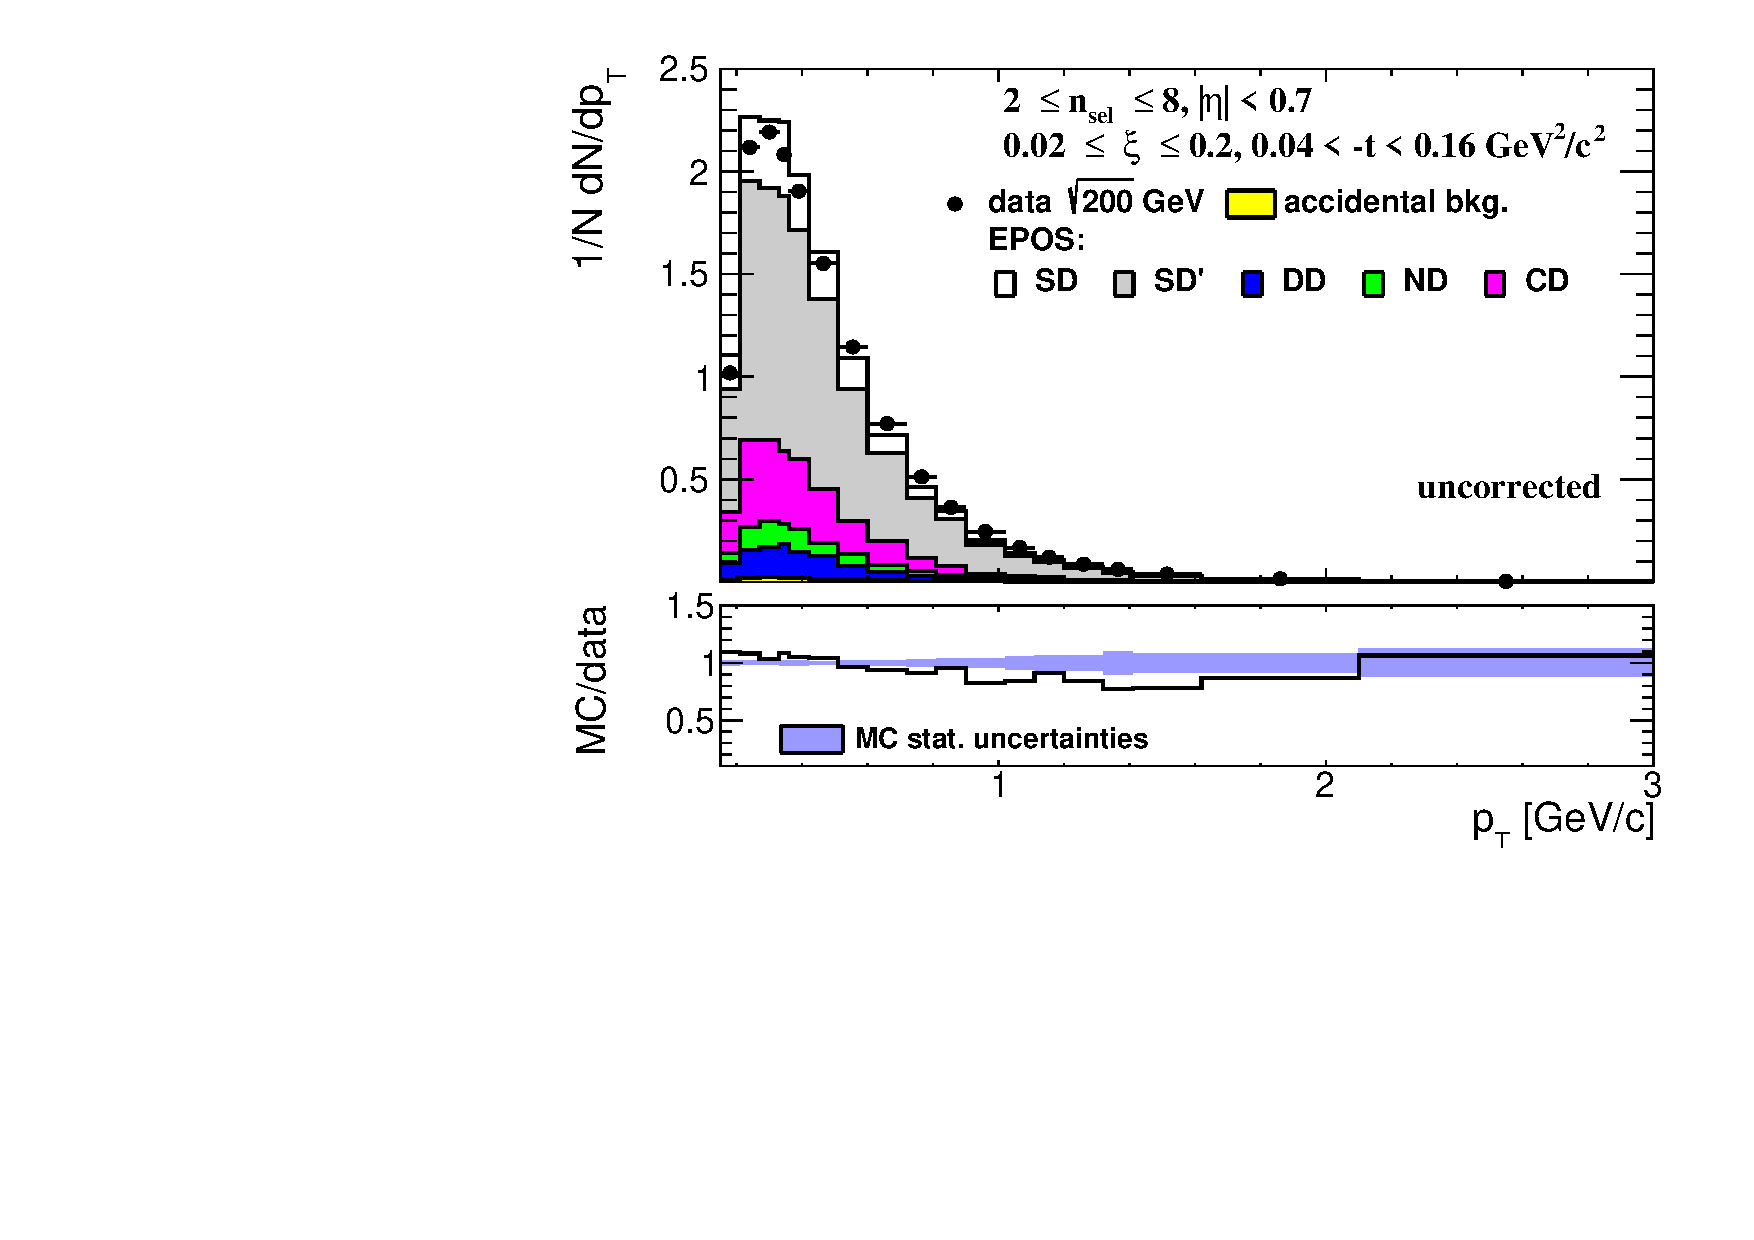
\includegraphics[width=\linewidth, page=1]{chapters/chrgSTAR/img/nonSD/chrg/SDT_epos_xi0_RP_starsim_pt.pdf}
	\end{subfigure}
	%\begin{minipage}{.49\textwidth}
		\caption{Uncorrected distributions of data compared to various MC models: (top left) PYTHIA~8 A2 (MBR), (top right) PYTHIA~8 A2 (MBR-tuned), (bottom left) PYTHIA~8 4C (SaS) and (bottom right) EPOS, as a function of $p_{\mathrm{T}}$. The~ratio of MC predictions and data is shown in the~bottom panels.}
		\label{fig:nonSDpt}
	%\end{minipage}
	%\vspace{-0.5cm}
\end{figure}
%\newpage
\begin{figure}[t!]
	%	\vspace{-0.5cm}
	\thisfloatpagestyle{fancy}
	\centering
	\begin{subfigure}{.49\textwidth}
		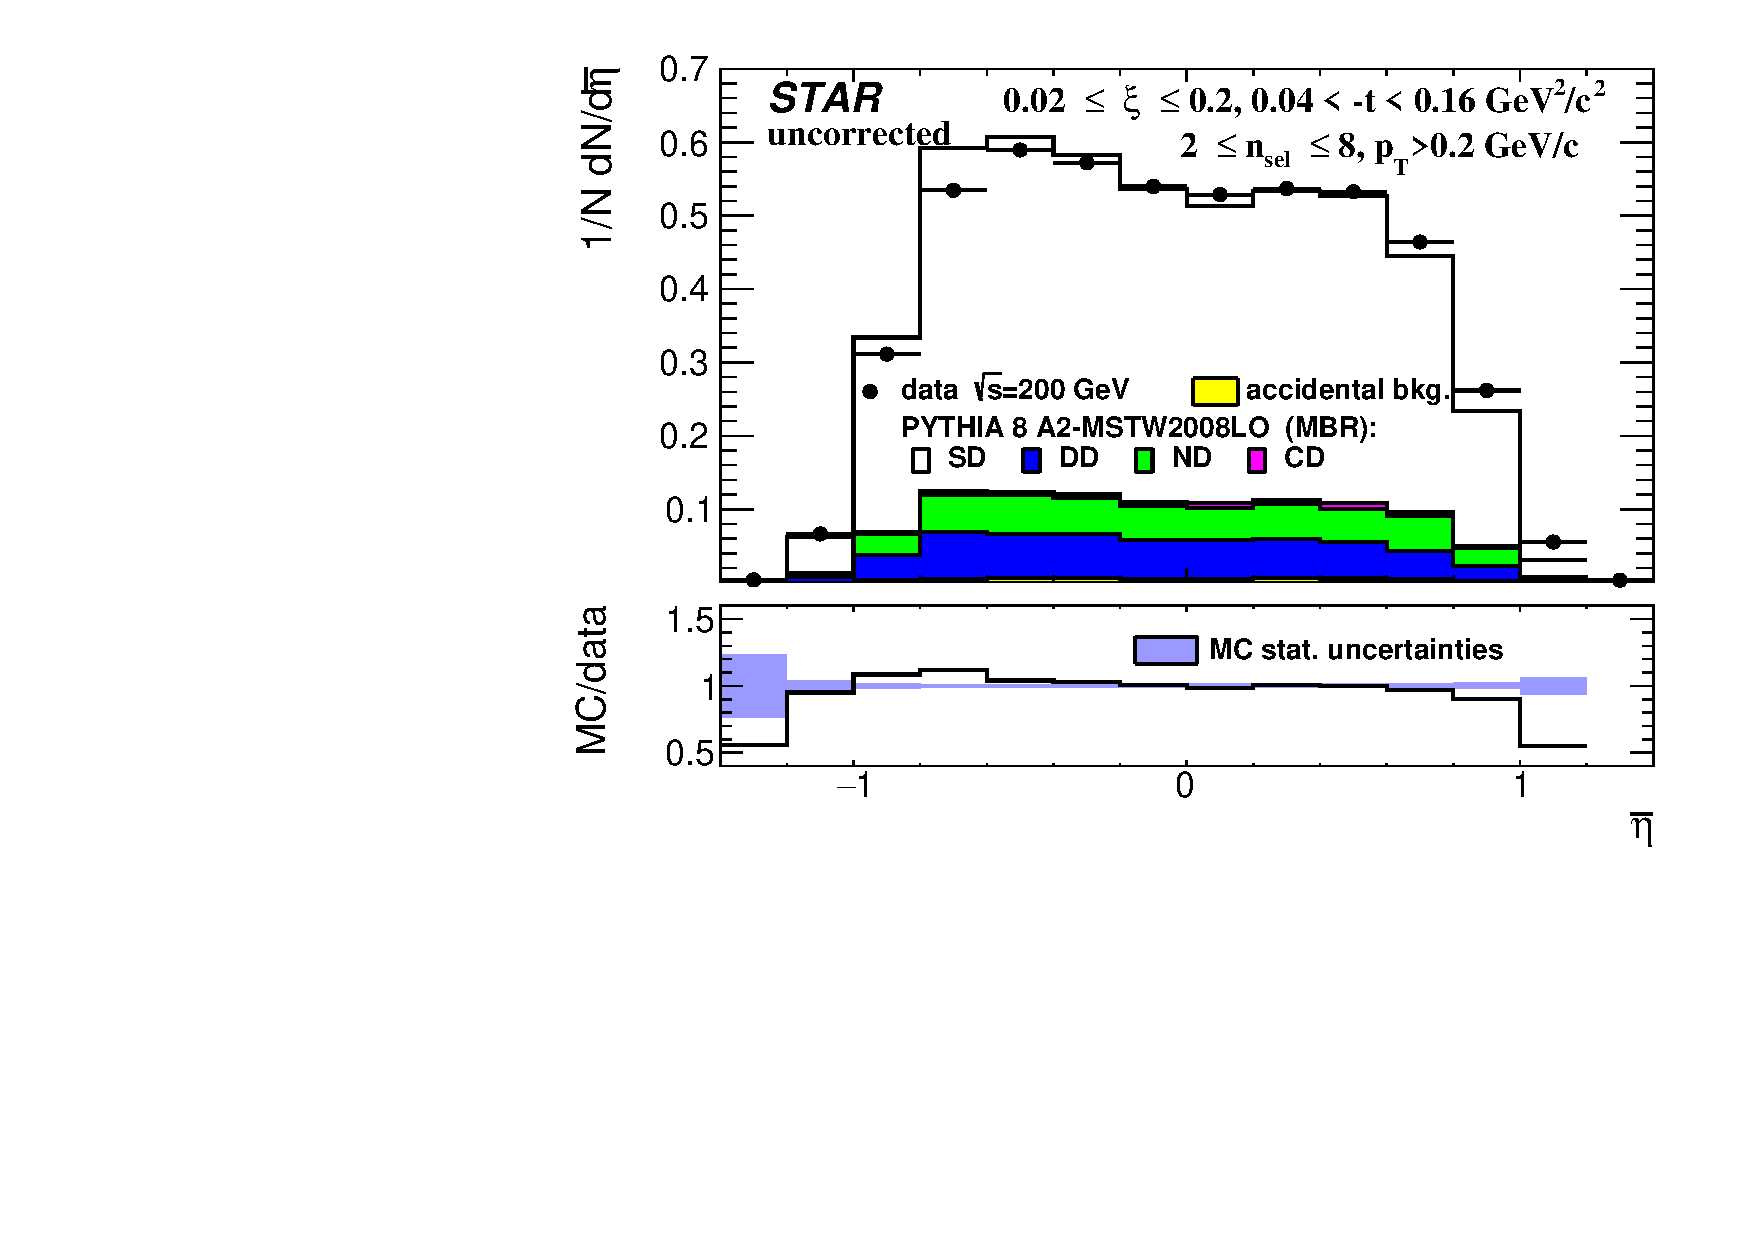
\includegraphics[width=\linewidth, page=1]{chapters/chrgSTAR/img/nonSD/chrg/SDT_pythia_xi0_RP_starsim_eta.pdf}
	\end{subfigure}
	\begin{subfigure}{.49\textwidth}
		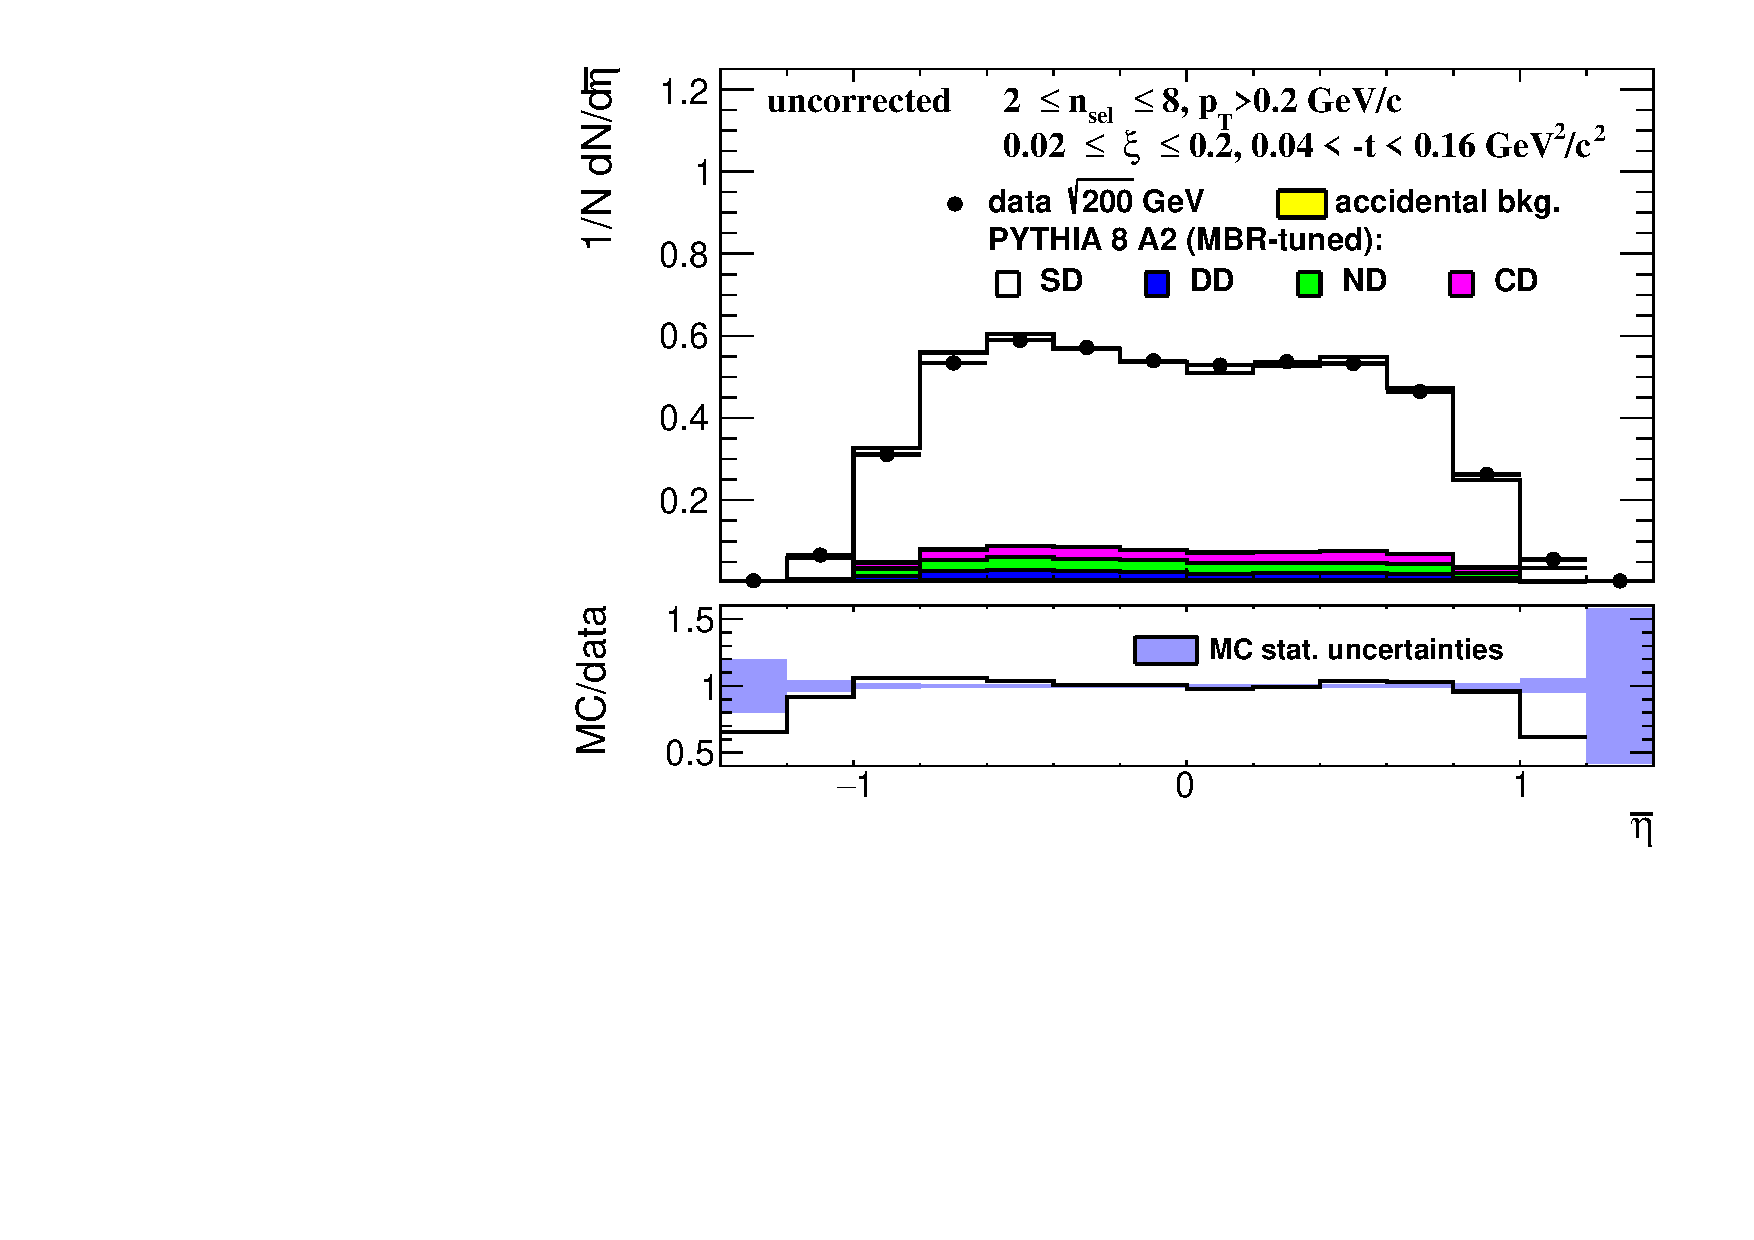
\includegraphics[width=\linewidth, page=1]{chapters/chrgSTAR/img/nonSD/chrg/SDT_pythia_xi0_option2_RP_starsim_eta.pdf}
	\end{subfigure}
	\begin{subfigure}{.49\textwidth}
		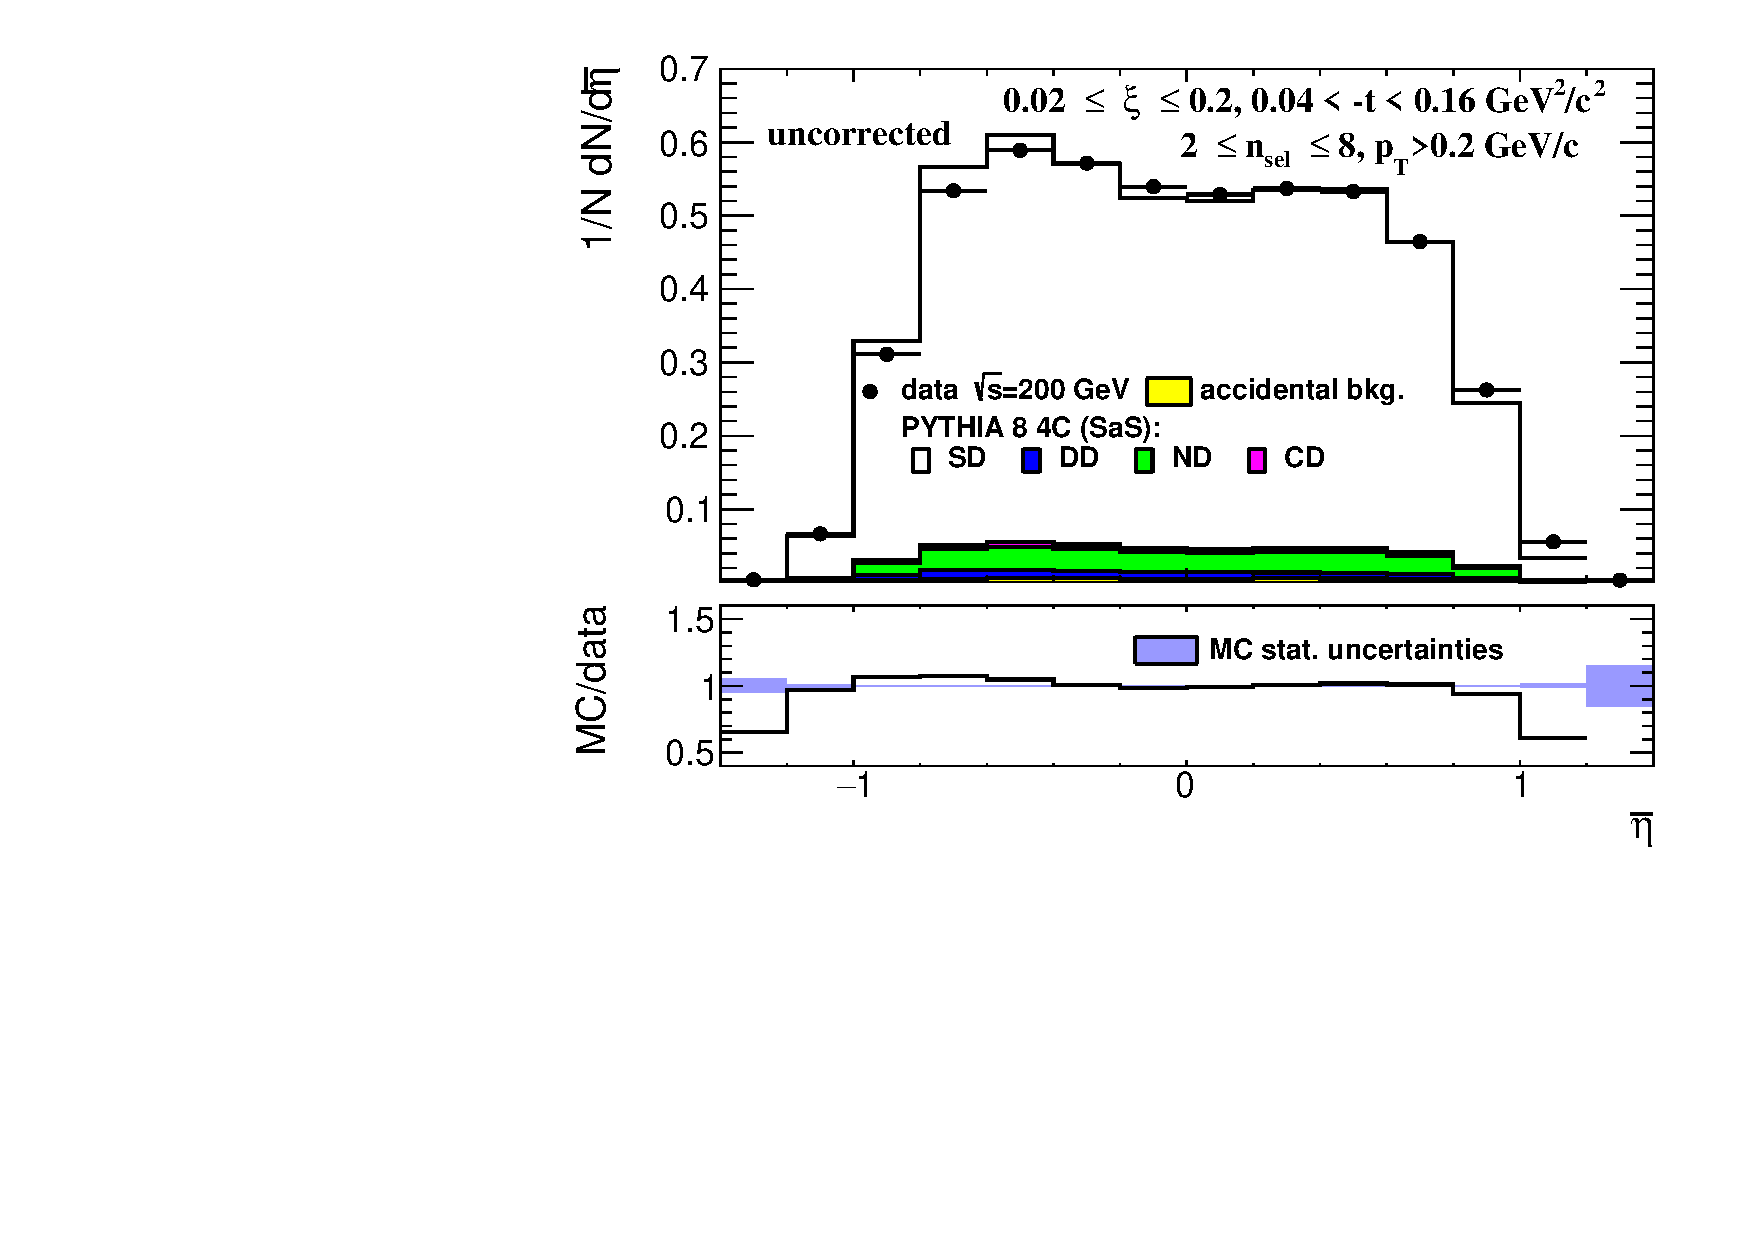
\includegraphics[width=\linewidth, page=1]{chapters/chrgSTAR/img/nonSD/SDT_pythia_xi0_sas_RP_starsim_eta.pdf}
	\end{subfigure}
	\begin{subfigure}{.49\textwidth}
		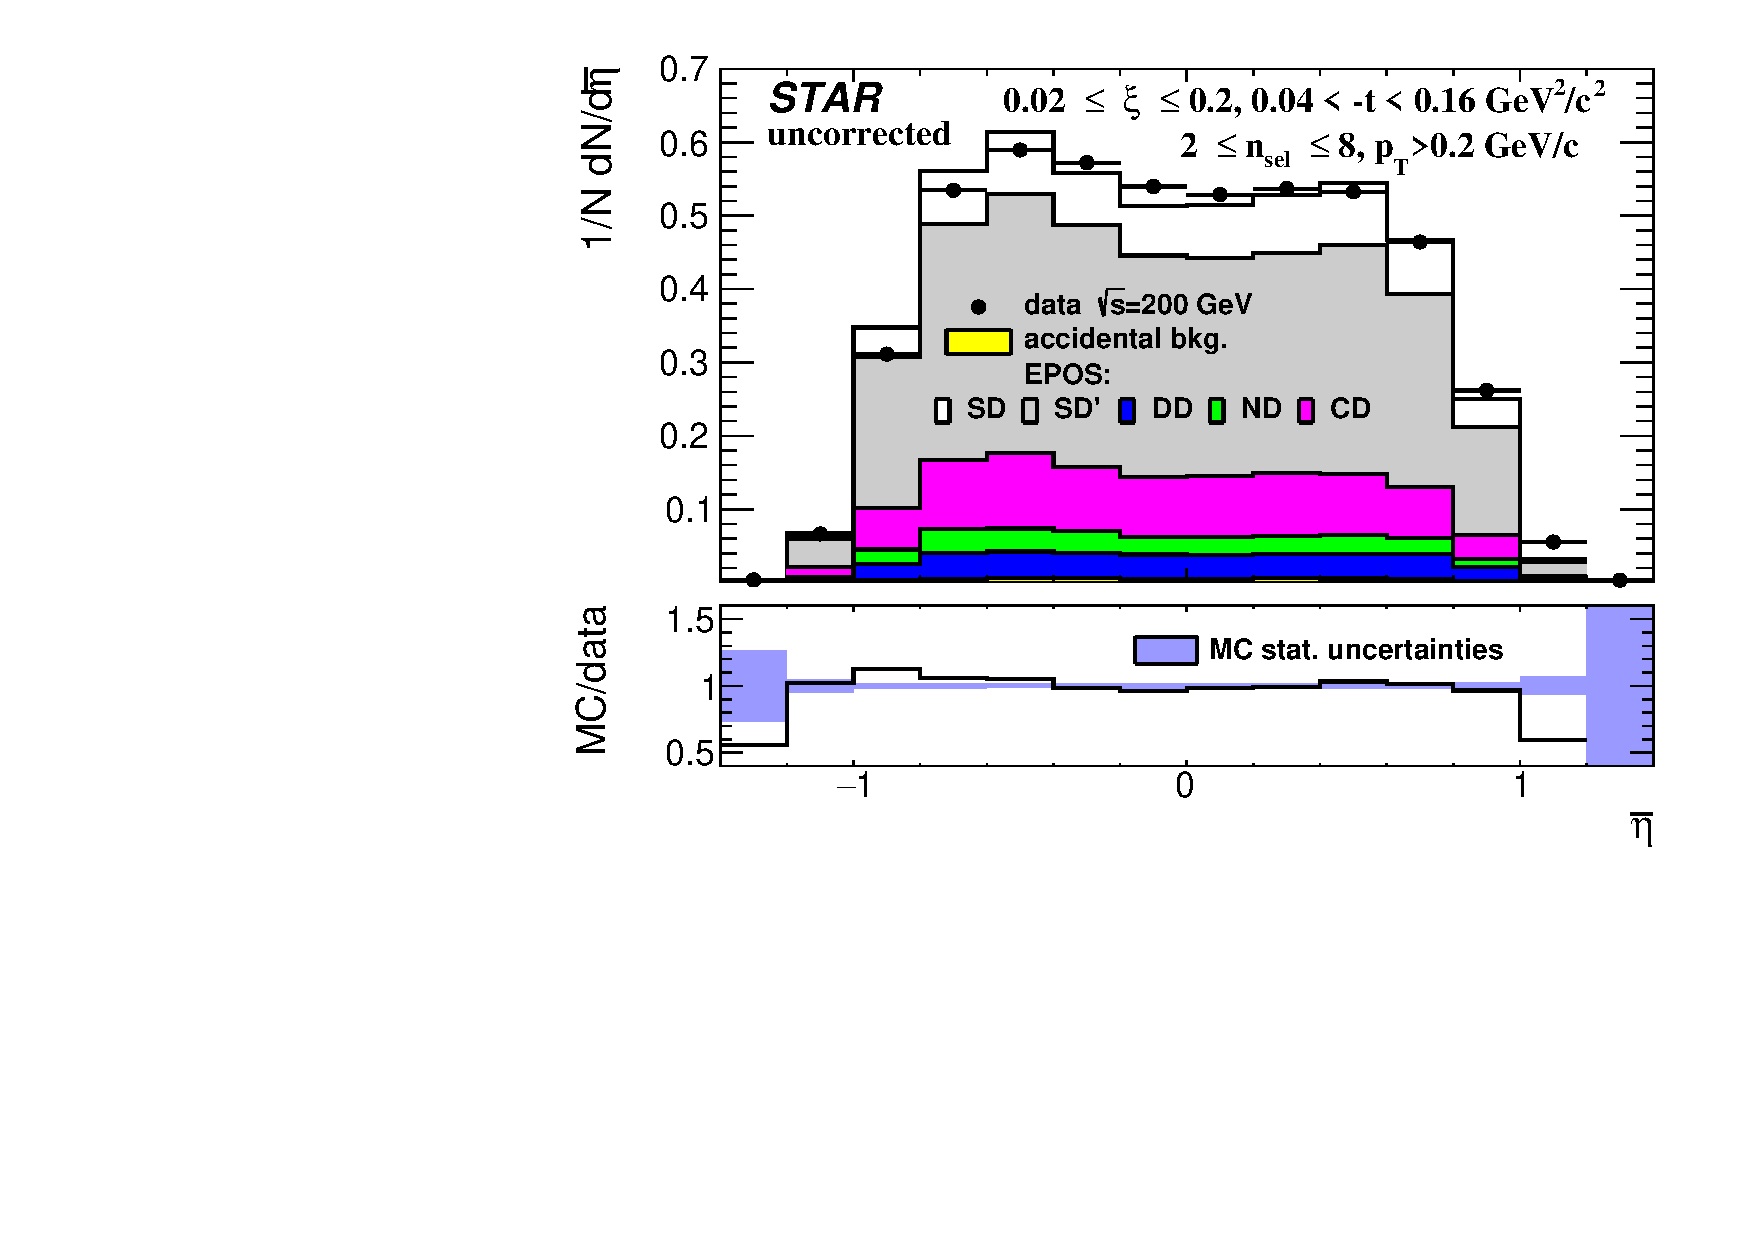
\includegraphics[width=\linewidth, page=1]{chapters/chrgSTAR/img/nonSD/chrg/SDT_epos_xi0_RP_starsim_eta.pdf}
	\end{subfigure}
	%\begin{minipage}{.49\textwidth}
		\caption{Uncorrected distributions of data compared to various MC models: (top left) PYTHIA~8 A2 (MBR), (top right) PYTHIA~8 A2 (MBR-tuned), (bottom left) PYTHIA~8 4C (SaS) and (bottom right) EPOS, as a function of $\bar{\eta}$. The~ratio of MC predictions and data is shown in the~bottom panels.}
		\label{fig:nonSDera}
	%\end{minipage}
	
\end{figure}
%\end{comment}
%\FloatBarrier